\documentclass[10pt,twocolumntoc]{cekarticle}
\usepackage{amsmath}
\usepackage{amssymb}
\usepackage{array}
\latexhtml{
  \usepackage[american]{varioref}
}{
  \newcommand{\vref}[1]{\ref{#1}}
}

% Aliases for bibliography entries, to compensate for some issues.

\defcitealias{bipm:1998}{BIPM, 1998}
\defcitealias{bipm:2000}{BIPM, 2000}


% Miscellaneous macros.

\newcommand{\D}{\displaystyle}
\newcommand{\tm}{\textsuperscript{\tiny{\texttrademark}}}
\newcommand{\changed}[1]{{#1}}
\newenvironment{blockChanged}{}

\pagestyle{myheadings}
\markboth{\textit{SBML Level 2: Working Draft Revision 3}}{\textit{SBML
    Level 2: Working Draft Revision 3}}



\begin{document}

%=============================================================================
% Title page
%=============================================================================

\title{Systems Biology Markup Language (SBML) Level 2:\\
  Structures and Facilities for Model Definitions}

\author{Andrew Finney, Michael Hucka}

\authoremail{\{afinney,mhucka\}@cds.caltech.edu}

\address{Systems Biology Workbench Development Group\\
  ERATO Kitano Symbiotic Systems Project\\
  Control and Dynamical Systems, MC 107-81\\
  California Institute of Technology, Pasadena, CA 91125, USA\\[3pt]
  \url{http://www.cds.caltech.edu/erato}}

\acknowledge{Principal Investigators: John Doyle and Hiroaki Kitano}

\date{SBML Level 2, Version 1\\[5pt]\fbox{Working Draft Revision 3}\\[5pt]
  \today{}}

\maketitlepage


%=============================================================================
\section{Introduction}
\label{sec:introduction}
%=============================================================================

We present the \textbf{S}ystems \textbf{B}iology \textbf{M}arkup
\textbf{L}anguage (SBML) Level~2, a model representation formalism for
systems biology.  SBML is oriented towards describing systems of
biochemical reactions common in research on a number of topics, including
cell signaling pathways, metabolic pathways, biochemical reactions, gene
regulation, and many others.  SBML is defined in a neutral fashion with
respect to programming languages and software encoding; however, it is
primarily oriented towards allowing models to be encoded using XML, the
eXtensible Markup Language~\citep{bosak:1999,bray:2000}.  This document
contains many examples of SBML models written in XML, as well as an XML
Schema~\citep{biron:2000,fallside:2000,thompson:2000} that defines SBML
Level~2.

Major releases of SBML are termed \emph{levels}.  SBML Level 2 evolved out
of SBML Level 1~\citep{hucka:2001}.  All of the structures of Level 1 can
be mapped in a straightforward fashion to Level~2.  In addition, a large
subset of the structures in Level~2 can be mapped to Level~1.  However, a
valid SBML Level~1 document is not a valid SBML Level~2 document or vice
versa.

SBML Level 2 was created in part studying the modeling facilities provided
by the following software systems: \emph{BioSpice}~\citep{arkin:2001},
\emph{Cellerator}~\citep{shapiro:2000,shapiro:2001,shapiro:2003},
\emph{COPASI}~\citep{mendes:2000},
\emph{DBSolve}~\citep{goryanin:2001,goryanin:1999},
\emph{E-Cell}~\citep{tomita:1999,tomita:2001},
\emph{Gepasi}~\citep{mendes:1997,mendes:2001},
\emph{Jarnac}~\citep{sauro:2000,sauro:1991},
\emph{JDesigner}~\citep{sauro:2001b},
\emph{JigCell}~\citep{vass:2003}, \emph{NetBuilder}~\citep{schilstra:2002},
\emph{ProMot/DIVA}~\citep{stelling:2001},
\emph{StochSim}~\citep{bray:2001,morton-firth:1998}, and \emph{Virtual
  Cell}~\citep{schaff:2000,schaff:2001}.  SBML was developed with the help
of the authors of these packages and with help and collaboration from the
authors of CellML~\citep{hedley:2001b}.

This SBML Level 2 specification document, the XML Schema corresponding to
SBML Level~2, and other related documents are openly available from the
SBML project web site, \url{http://www.sbml.org/}.


%-----------------------------------------------------------------------------
\subsection{Scope and Limitations}
%-----------------------------------------------------------------------------

SBML Level 2 is meant to support non-spatial biochemical models and the
kinds of operations that are possible in existing analysis/simulation
tools.  Future software tools will undoubtedly require further evolution of
SBML; we expect that subsequent levels will add additional structures and
facilities currently missing from Level~2, once the simulation community
gains experience with the current language definition. In
Section~\ref{sec:level-3}, we discuss extensions that will likely be
included in SBML Level~3.

The definition of the model description language presented here does not
specify \emph{how} programs should communicate or read/write SBML.  We
assume that for a simulation program to communicate a model encoded in
SBML, the program will have to translate its internal data structures to
and from SBML, use a suitable transmission medium and protocol, etc., but
these issues are outside of the scope of this document.

%-----------------------------------------------------------------------------
\subsection{Differences between Level 1 Version 1 and Level 2}
%-----------------------------------------------------------------------------

Compared to SBML Level 1 Version 1, SBML Level 2 introduces the following
changes: 
\begin{itemize}
  
\item SBML Level 2 supports the inclusion of metadata using the same approach as
  CellML~\citep{cuellar:2002}.  All structures in SBML can be annotated
  with optional content in RDF~\cite[Resource Description
  Format;][]{lassila:1999} following the guidelines put forward by
  \citeauthor{cuellar:2002}  See Section~\ref{sec:sbase}.
  
\item A new field called \attrib{id} replaces the \attrib{name} field
  previously defined for most SBML structures to identify components in a
  model.  The new \attrib{id} field has a type of \class{SId}, whose
  definition is similar to \class{SName} in Level~1; see
  Section~\ref{sec:idnameattribs}.  In SBML Level~2, the \attrib{name}
  field has become optional and has been redefined to allow any Unicode
  characters allowed by the \class{string} type of XML
  Schema~\citep{biron:2000}.  The combination of \attrib{id} and
  \attrib{name} allows software tools to use meaningful names for
  components in a model, while simultaneously preserving the ability of
  software tools that cannot display special characters to display and
  manipulate \emph{some} sort of labels for those components.
  
\item Formulas in Level~2 are expressed using MathML~\citep{w3c:2000b}.
  The field named \attrib{formula} previously available on the
  \class{KineticLaw} and \class{Rule} structures has been replaced by a
  MathML element named \class{math} containing MathML content; see
  Sections~\ref{sec:formulas}, \ref{sec:rules}
  and~\ref{subsec:kinetic-law}.  The subset of MathML used in SBML includes
  logical operators enabling the expression of discontinuous functions,
  something that was not possible in SBML Level~1.
  
\item All attributes which contain initial conditions or parameter values,
  including compartment volumes and species concentrations,
  are optional in Level~2 rather than, as in Level~1, either being mandatory
  or having default values. A missing attribute value for one of these attributes
  implies that the value is either unknown, not required for analysis, or should be obtained
  from an external source; see Sections~\ref{sec:compartments}, \ref{sec:species} and \ref{sec:parameters}.
  
\item The top-level \class{Model} structure can contain an optional list of
  global function definitions expressed in MathML and organized in new
  structures of type \class{FunctionDefinition}.  See
  Sections~\ref{sec:formulas} and \ref{sec:functions}.
  
\item The top-level \class{Model} structure can contain an optional list of
  events organized in structures of type \class{Event} which specify the a
  discrete event can occur during a simulation. See Section \ref{sec:events}.
  
\item The namespace for identifiers in a model does not contain any
  built-in symbols; gone, for example, are the predefined rate laws of SBML
  Level~1.  The approach taken in SBML Level~2 is that each model must
  itself define whatever functions it uses using the new
  \class{FunctionDefinition} mechanism.  Although SBML Level~2 uses a
  feature of MathML to allow models to refer to two particular built-in
  entities (a symbol representing time and another symbol representing
  delay functions), even these entities are not in the same namespace as
  the model's identifiers.  See Section~\ref{sec:mathmltokens}.
  
\item Species, compartments and reactions are each optional in a model;
  thus, a model does not need to contain species, compartments or reactions
  to be valid.  See section~\ref{sec:model}.
  
\item The \class{Compartment}, \class{Species} and \class{Parameter}
  structures each have a new boolean field named \attrib{constant}.  This
  field specifies whether the variables represented by these structures
  can be changed by rules and reactions.  See
  Sections~\ref{sec:compartments}, \ref{sec:species}
  and~\ref{sec:parameters}.
 
\item SBML Level~2 specifies certain constraints on the form and use of
  scalar rules in order to prevent such things as algebraic loops.  See
  Section~\ref{sec:rules}.
  
\item \class{Rule} structures have been changed and simplified.  Instances of
  \class{AssignmentRule} replace instances of \class{ParameterRule},
  \class{SpeciesConcentrationRule} and \class{CompartmentVolumeRule}.
  See Section~\ref{sec:rules}.
  
\item A rule is not a substitute for a component definition.  For example,
  a \class{Compartment} structure for a given identifier must precede an
  \class{AssignmentRule} structure for the same identifier.
  
\item A new \attrib{listOfModifiers} element has been added to the
  \class{Reaction} structure.  This list enumerates species that affect a
  reaction but are neither created nor destroyed by the reaction.  Each species
  occurring in a kinetic law must appear in the list of reactants, list of
  products or list of modifiers. See Section~\ref{sec:reactions}.
  
\item A reaction may have no products or no reactants but must have at
  least one reactant or product.  See Section~\ref{sec:reactions}.
  
\item The word \emph{specie} has been replaced in all instances by
  \emph{species}.

\item Unlike in SBML Level 1, unit identifiers in Level~2 are in a separate
  namespace from the namespace used for models, functions, species,
  compartments, reactions and parameters.
  
\item All structures, including \class{Sbml} and
  \class{listOf}\rule{0.5in}{0.5pt} elements, are derived from the base
  type \class{SBase}.

\end{itemize}

%-----------------------------------------------------------------------------
\subsection{Notational Conventions}
%-----------------------------------------------------------------------------

We define SBML using a graphical notation based upon UML, the Unified
Modeling Language~\citep{eriksson:1998,oestereich:1999}.  This UML-based
definition in turn is used to define an XML
Schema~\citep{biron:2000,fallside:2000,thompson:2000} for SBML.  There are
three main advantages to using UML as a basis for defining SBML data
structures.  First, compared to using other notations or a programming
language, the UML visual representations are generally easier to grasp by
readers who are not computer scientists.  Second, the visual notation is
implementation-neutral: the defined structures can be encoded in any
concrete implementation language---not just XML, but C or Java as well.
Third, UML is a de facto industry standard that is documented in many
sources.  Readers are therefore more likely to be familiar with it than
other notations.

Our notation and our approach for mapping it to XML Schemas is explained in
a separate document~\citep{hucka:2000b}.  A summary of the essential points
is presented in Appendix~\ref{apdx:notation}, and examples throughout this
document illustrate the approach.  We also follow certain naming and
typographical conventions throughout this document.  Specifically, the
names of data structure attributes or fields begin with a lowercase letter,
and the names of data structures and types begin with an uppercase letter.
Keywords (names of types, XML elements, etc.) are written in a
typewriter-style font; for example, \class{Compartment} is a type name and
\class{compartment} is a field name.  Likewise, literal XML examples are
also written in a typewriter-style font.


%=============================================================================
\section{Overview of SBML}
\label{sec:overview}
%=============================================================================

The following is an example of a simple, hypothetical network of
biochemical reactions that can be represented in SBML:
\begin{equation*}
  \begin{array}{@{}ccl@{}}
    S_1 & \underrightarrow{k_1 [S_1] / ([S_1] + k_2)} & S_2 \\ \\[-3pt]
    S_2 & \underrightarrow{k_3 [S_2]} & S_3 + S_4
  \end{array}
\end{equation*}
Broken down into its constituents, this model contains a number of
components: reactant species, product species, reactions,
rate laws, and parameters in the rate laws.  To analyze or
simulate this network, additional components must be made
explicit, including compartments for the species, and units on the
various quantities.  The top level of an SBML model definition
simply consists of lists of these components:
\begin{center}
  \slshape
  \begin{tabular}{c}
    \begin{minipage}{3in}
      \begin{tabbing}
        xxxx\=xxxx\=xxxx\=xxxx\=\kill
        beginning of model definition\\
        \>list of function definitions (optional)\\
        \>list of unit definitions (optional)\\
        \>list of compartments (optional)\\
        \>list of species (optional)\\
        \>list of parameters (optional)\\
        \>list of rules (optional)\\
        \>list of reactions (optional)\\
        \>list of events (optional)\\
        end of model definition
      \end{tabbing}
    \end{minipage}
  \end{tabular}
\end{center}
The meaning of each component is as follows:
\begin{description}

\item \emph{Function definition}: A named function that may be used
  throughout the rest of the model.
    
\item \emph{Unit definition}: A name for a unit used in the expression of
  quantities in a model.  Units may be supplied in a number of contexts in
  an SBML model, and it is convenient to have a facility for both setting
  default units and for allowing combinations of units to be given
  abbreviated names.

\item \emph{Compartment}: A container of finite volume for substances.  In
  SBML Level~2, a compartment is primarily a topological structure with a
  volume but no geometric qualities.
  
\item \emph{Species}: A substance or entity that takes part in a reaction.
  Some example species are ions such as $\text{Ca}^{2+}$ and molecules such
  as glucose or ATP.  The primary qualities associated with a chemical
  species in SBML Level~2 are its initial amount and the compartment in
  which it is located.
  
\item \emph{Parameter}: A quantity that has a symbolic name.  SBML Level~2
  provides the ability to define parameters that are global to a model as
  well as parameters that are local to a single reaction.
 
\item \emph{Rule}: In SBML, a mathematical expression that is used in
  combination with the differential equations constructed based on the set
  of reactions; it can be used to establish constraints between variables in
  a model, define how a variable can be calculated from other variables,
  or used to define the rate of change of a variable.

\item \emph{Reaction}: A statement describing some transformation,
  transport or binding process that can change the amount of one or more
  species.  For example, a reaction may describe how certain entities
  (reactants) are transformed into certain other entities (products).
  Reactions have associated rate laws describing how quickly they take
  place.
  
\item \emph{Event}: A statement describing an instantaneous, discontinuous
  transformation of a set of variables of any type (species concentration,
  compartment volume or parameter value) when some triggering condition is
  satisfied. 
\end{description}

A software package can read an SBML model description and translate it
into its own internal format for model analysis.  For example, a package
might provide the ability to simulate the model by constructing
differential equations representing the network and then performing
numerical time integration on the equations to explore the model's dynamic
behavior.

SBML allows models of arbitrary complexity to be represented.  Each type of
component in a model is described using a specific type of data structure
that organizes the relevant information.  The data structures determine how
the resulting model is encoded in XML.

In the sections that follow, the various constructs in SBML and their uses
are described in detail.  Section~\ref{sec:general} first introduces a few
basic structures that are used throughout SBML Level~2, then
Section~\ref{sec:elements} provides details on each of the main components.
Section~\ref{sec:xml-rep} provides a number of complete examples of models
encoded in XML using SBML Level~2.  Section~\ref{sec:discussion} contains a
list of anticipated enhancements that will be made in SBML Level 3 and a
discussion of other efforts related to SBML.  Appendix~\ref{apdx:schema}
provides the complete XML Schema for SBML Level~2.


%=============================================================================
\section{Preliminary Definitions}
\label{sec:general}
%=============================================================================

This section covers certain concepts and constructs that are used
repeatedly in the rest of SBML Level 2 and are useful to discuss before
diving into the details of the components provided in SBML Level 2.

%-----------------------------------------------------------------------------
\subsection{Type \class{SBase}}
\label{sec:sbase}
%-----------------------------------------------------------------------------

Each of the main structures composing an SBML Level 2 model definition has
a specific data type that is derived directly or indirectly from a single
abstract type called \class{SBase}.  This inheritance hierarchy is depicted
in Figure~\vref{fig:top-level}.  In addition to this, all the
\class{listOf}\rule{0.5in}{0.5pt}\class{s} elements in SBML are derived
from \class{SBase}.

\begin{figure}[ht]
  \vspace*{8pt}
  \centering
  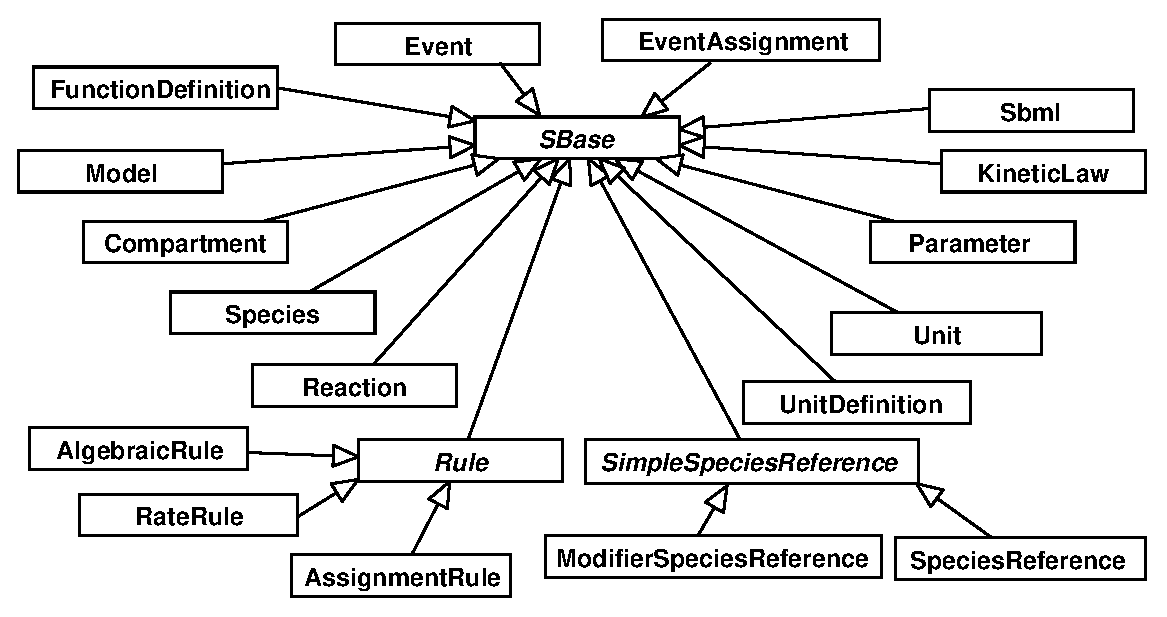
\includegraphics[scale = 0.7]{top-level}
  \caption{A UML diagram of the inheritance hierarchy of major data types
    in SBML.  Open arrows indicate inheritance, pointing from inheritors to
    their parents~\citep{eriksson:1998,oestereich:1999}.}
  \label{fig:top-level}
\end{figure}

\begin{figure}[ht]
  \centering
  
\includegraphics[scale = 0.68]{identified}
  \caption{The definition of \class{SBase}.  Text enclosed in braces next
    to attribute types (e.g., \attribtype{\{minOccurs="0"\}}) indicates
    constraints on the possible attribute values.  We use XML Schema
    language to express constraints since we are primarily interested in
    the XML encoding of SBML.  The constraint expression
    \attribtype{use="optional"} means that the indicated field is optional
    and may be omitted in a particular instance in a model.  The constraint
    expression \attribtype{minOccurs="0"} likewise means that the indicated
    field is optional; the alternate form must be used in XML Schema for
    those fields that are containers (i.e., fields that are encoded as
    subelements in XML).}
  \label{fig:sbase}
\end{figure}

The type \class{SBase} is designed to allow a modeler or a software package
to attach arbitrary information to each major component in an SBML model.
The definition of \class{SBase} is presented in Figure~\vref{fig:sbase}.
\class{SBase} contains three fields, all of which are optional:
\attrib{metaid}, \attrib{notes} and \changed{\attrib{annotation}}.

The \attrib{metaid} field is present for supporting metadata annotations
using RDF.  It has a data type of \class{ID} (the XML identifier type), and
serves as anchors for metadata references.  Metadata expressed using RDF
can be placed anywhere within an \class{sbml} element and its subelements,
\emph{except} within MathML elements.  The metadata elements can include
RDF \class{description} elements in which the RDF \attrib{describes}
attributes contain the values of the \attrib{metaid} fields of SBML
elements in the model.  The form of the RDF element content in SBML should
follow the form described in the CellML Metadata
Specification~\citep{cuellar:2002}.

The field \attrib{notes} in \class{SBase} is a container for XHTML content.
It is intended to serve as a place for storing optional information
intended to be seen by humans.  An example of the kind of information that
would be appropriate to place inside \attrib{notes} is user comments about
a particular component of the model.  Every data object derived directly or
indirectly from type \class{SBase} can have a separate value for
\attrib{notes}, allowing users considerable freedom for annotating their
models.  A software tool that reads and manipulates SBML is expected to
provide some mechanism for displaying the contents of \attrib{notes} fields
in a model.

Finally, \class{SBase} includes the field called \attrib{annotation} to
provide a container for software-generated annotations that are \emph{not}
intended to be seen by humans.  This field is a container for arbitrary
data (XML type \class{any}).  As with the user-visible \attrib{notes}
field, every data object can have its own value for \attrib{annotation}.
Guidelines for using this field are given in the next section.

In the other SBML type definitions presented below, we follow the UML
convention of hiding the attributes derived from a parent type such as
\class{SBase}. It should be kept in mind that these attributes are always
available.


%-----------------------------------------------------------------------------
\subsection{Guidelines for the Use of the \attrib{annotation} Field in
  \class{SBase}}
%-----------------------------------------------------------------------------

The \attrib{annotation} field in the definition of \class{SBase} is
formally unconstrained in order that software developers may attach any
information they need to different components in an SBML model. However,
it is important that this facility not be misused accidentally.  In
particular, it is critical that information essential to a model definition
is \emph{not} stored in \attrib{annotation}.  Parameter values, functional
dependencies between model components, etc., should not be recorded as
annotations.

Here are examples of the kinds of data that may be appropriately
stored in \attrib{annotation}: (a) Information about graphical
layout of model components; (b) application-specific processing
instructions that do not change the essence of a model; (c)
identification information for cross-referencing components in a
model with items in a database.

Different applications may use XML Namespaces~\citep{bray:1999} to specify
the intended vocabulary of a particular annotation.  Here is an example.
Suppose a particular application needs to annotate data structures in
an SBML model definition with screen layout information and a time stamp.
The application's developers should choose a URI (\emph{Universal Resource
  Identifier}; \citealt{harold:2001,w3c:2000}) reference that uniquely
identifies the vocabulary that the application will use for such
annotations, and a prefix string to be used in the annotations.  For
illustration purposes, let us say the URI reference is
``\texttt{http://www.mysim.org/ns}'' and the prefix is \texttt{mysim}.  An
example of an annotation might then be:

\begin{example}
...
<annotation xmlns:mysim="http://www.mysim.org/ns">
    <mysim:nodecolors mysim:bgcolor="green" mysim:fgcolor="white"/>
    <mysim:timestamp>2000-12-18 18:31 PST</mysim:timestamp>
</annotation>
...
\end{example}

The namespace prefix \texttt{mysim} is used to qualify the XML elements
\texttt{mysim:nodecolors} and \texttt{mysim:timestamp}; presumably these
symbols have meaning to the application.  This example places the XML
Namespace information on \attrib{annotation} itself rather than on a
higher-level enclosing construct or the enclosing document level, but other
placements would be valid as well~\citep{bray:1999}.

\begin{table}[b]
  \vspace*{10pt}
  \small
  \centering
  \begin{tabular}{ll}
    \toprule
    \texttt{http://www.sbml.org/2001/ns/basis}      & \texttt{http://www.sbml.org/2001/ns/jdesigner}\\
    \texttt{http://www.sbml.org/2001/ns/biocharon}  & \texttt{http://www.sbml.org/2001/ns/jigcell}\\
    \texttt{http://www.sbml.org/2001/ns/bioreactor} & \texttt{http://www.sbml.org/2001/ns/jsim}\\
    \texttt{http://www.sbml.org/2001/ns/biosketchpad}   & \texttt{http://www.sbml.org/2001/ns/mcell}\\
    \texttt{http://www.sbml.org/2001/ns/biospice}   & \texttt{http://www.sbml.org/2001/ns/moma}\\
    \texttt{http://www.sbml.org/2001/ns/cellerator} & \texttt{http://www.sbml.org/2001/ns/netbuilder}\\
    \texttt{http://www.sbml.org/2001/ns/copasi}     & \texttt{http://www.sbml.org/2001/ns/pathdb}\\
    \texttt{http://www.sbml.org/2001/ns/cytoscape}  & \texttt{http://www.sbml.org/2001/ns/promot}\\
    \texttt{http://www.sbml.org/2001/ns/dbsolve}    & \texttt{http://www.sbml.org/2001/ns/sbedit}\\
    \texttt{http://www.sbml.org/2001/ns/ecell}      & \texttt{http://www.sbml.org/2001/ns/stochsim}\\
    \texttt{http://www.sbml.org/2001/ns/gepasi}     & \texttt{http://www.sbml.org/2001/ns/vcell}\\
    \texttt{http://www.sbml.org/2001/ns/isys}       & \texttt{http://www.sbml.org/2001/ns/winscamp}\\
    \texttt{http://www.sbml.org/2001/ns/jarnac} \\
    \bottomrule
  \end{tabular}
  \caption{Reserved XML Namespace names in SBML Level 2.}
  \label{tab:reserved-urls}
\end{table}

The use of XML Namespaces permits multiple applications to place
annotations on SBML elements without risking interference or element name
collisions.  Annotations stored by different simulation packages can thus
coexist in the same model definition.  Although XML Namespace names
(``\texttt{http://www.mysim.org/}'' in the example above) must be URI
references, an XML Namespace name is \emph{not required} to be directly
usable in the sense of identifying an actual, retrieval document or
resource on the Internet~\citep{bray:1999}.  The name is simply intended to
enable unique identification of constructs, and using URIs is a common and
simple way of creating a unique name string.  For the convenience of the
simulation community, we reserve certain namespace names for use with
annotations in SBML.  These reserved names are listed in
Table~\ref{tab:reserved-urls}.

Note that the namespaces being referred to here are XML Namespaces
specifically in the context of the \attrib{annotation} field on
\class{SBase}.  The namespace issue here is unrelated to the namespaces
discussed in Section~\ref{sec:namespaces} in the context of
\class{SName} and symbols in SBML.

%-----------------------------------------------------------------------------
\subsection{\attrib{id} and \attrib{name} attributes on SBML components}
\label{sec:idnameattribs}
%-----------------------------------------------------------------------------

As will become apparent below, nearly all structures in SBML include two
particular fields: \attrib{id} and \attrib{name}.  The \attrib{id} field is
required and is used to identify a component within the model definition.
Other SBML structures refer to the component using this identifier.  The
next section defines the data type \class{SId} used for the \attrib{id}
field, and Section~\ref{sec:namespaces} describes the scoping and namespace
rules for these identifiers.

In contrast to the \attrib{id} field, the \attrib{name} field is optional.
Its data type is the type \class{string} defined in XML
Schema~\citep{biron:2000,thompson:2000}, which includes all Unicode
characters~\citep{unicode:1996} except for two delimiter characters, 0xFFFE
and 0xFFFF~\citep{biron:2000}.  The purpose of the \attrib{name} field is
to provide a human-readable label for the component.  No restrictions as to
its contents are imposed by SBML beyond those defined by the \class{string}
type of XML Schema.

The recommended practice for handling \attrib{name} is as follows.  If a
software tool has the capability for displaying the content of
\attrib{name} fields, it should display this content to the user as a
component's label instead of the component's \attrib{id} field.  If the
user interface does not have this capability (e.g., because it cannot
display special characters), or if the \attrib{name} field is missing on a
given component, then the user interface should display the value of the
\attrib{id} field.  (Script language interpreters are especially likely to
display \attrib{id} fields instead of \attrib{name} fields.)

As a consequence of the above, authors of systems that automatically
generate the values of \attrib{id} fields should be aware some systems may
display the \attrib{id}'s to the user.  Authors may wish to take some care
to have their software create \attrib{id} values that are easy for humans
to type and read.

%-----------------------------------------------------------------------------
\subsection{Type \class{SId}}
\label{sec:id}
%-----------------------------------------------------------------------------

The type \class{SId} is the type of the \attrib{id} field found on the
majority of SBML components.  \class{SId} is a data type derived from the
basic XML type \class{string}, but with restrictions about the types of
characters permitted and the sequence in which they may appear.  Its
definition is shown in Figure~\vref{fig:id}.

\begin{figure}[ht]
  \vspace*{5pt}
  \centering
  \begin{minipage}{3.8in}
\begin{verbatim}
  letter ::= 'a'..'z','A'..'Z'
  digit  ::= '0'..'9'
  nameChar ::= letter | digit | '_'
  name ::= ( letter | '_' ) nameChar*
\end{verbatim}
  \end{minipage}
  \caption{The definition of the type \class{SId} expressed in the variant
    of XML used by the XML 1.0 specification~\protect\citep{bray:2000}.
    The characters \texttt{(} and \texttt{)} are used for grouping, and the
    character \texttt{*} indicates ``zero or more times''.}
  \label{fig:id}
\end{figure}

The \class{SId} is purposefully not derived from the XML \class{ID} type.
Doing so would force all SBML identifiers to exist in a single global
namespace, which would affect not only the form of local parameter
definitions but also future extensions for supporting model/submodel
composition.  Further, the use of the \class{ID} type for SBML identifiers
would have limited utility because MathML \class{ci} elements are not of
the type \class{IDREF} (see Section~\ref{sec:formulas}).  If the
\class{IDREF}-\class{ID} linkage cannot be exploited in MathML constructs,
the utility of the XML \class{ID} type is greatly reduced.

%The type \class{SLocalId} is used in types where a component
%identifier does not have global scope thus \class{SLocalId} has
%the same syntax as \class{SId} but is derived from XML type
%{string}.

%-----------------------------------------------------------------------------
\subsection{Component Identifiers and Namespaces in SBML}
\label{sec:namespaces}
%-----------------------------------------------------------------------------

A biochemical network model can contain a large number of
components representing different parts of a model.  This leads to
a problem in deciding the scope of an identifer: in what contexts
does a given identifier \emph{X} represent the same thing?  The
approaches used in existing simulation packages tend to fall into
two categories that we may call global and local.  The
\emph{global} approach places all identifiers into a single global
namespace, so that an identifier \emph{X} represents the same thing
wherever it appears in a given model definition.  The \emph{local}
approach places symbols in different namespaces depending on the
context, where the context may be, for example, individual rate
laws.  The latter approach means that a user may use the same
identifer \emph{X} in different rate laws and have each instance
represent a different quantity.

The fact that different simulation programs may use different
rules for identifier resolution poses a problem for the exchange
of models between simulation tools.  Without careful
consideration, a model written out in SBML format by one program
may be misinterpreted by another program.  SBML Level 2 must
therefore include a specific set of rules for treating identifer
and namespaces.

The namespace rules in SBML Level 2 are relatively straightforward
and are intended to avoid this problem with a minimum of
requirements on the implementation of software tools:
\begin{itemize}
  
\item The identifiers of functions, compartments, species, reactions,
  events and model-level parameters reside in the same global namespace.
  This means, for example, that a reaction and a species definition cannot
  both have the same identifier.
  
\item Each reaction definition (see Section~\ref{sec:reactions})
  establishes a private local namespace for local parameter identifiers.
  Within the definition of a given reaction, local parameter identifiers
  introduced in that reaction override (shadow) identical identifers in the
  global namespace.
  
\item Unit names exist in a separate global namespace from other
  identifiers.

\end{itemize}

The set of rules above can enable software packages using either
local or global namespaces for parameters to exchange SBML model definitions.
In particular, software environments using local namespaces for parameters
internally should be able to accept SBML model definitions without
needing to change component identifiers. Environments using a
global namespace for parameters internally can perform a simple manipulation of
the identifiers of local parameter elements within reaction definitions to
avoid name collisions.  (An example approach for the latter would be the
following: when receiving an SBML-encoded model, prefix each
parameter identifier inside each reaction with a string constructed from the
reaction's identifier; when writing an SBML-encoded model, strip
off the prefix.)

The namespace rules described here provide a clean transition path
to future levels of SBML, when submodels are introduced
(Section~\ref{sec:level-3}).  Submodels will provide the ability
to compose one model from a collection of other models.  This
capability will have to be built on top of SBML Level~2's
namespace organization.  A straightforward approach to handling
namespaces is to make each submodel's space be private.  The rules
governing namespaces within a submodel can simply be the Level~2
namespace rule described here, with each submodel having its own
(to itself, global) namespace.

%-----------------------------------------------------------------------------
\subsection{Mathematical Formulas in SBML Level 2}
\label{sec:formulas}
%-----------------------------------------------------------------------------

Math in SBML Level 2 is expressed using MathML~\citep{w3c:2000b}.  MathML is
used in the definitions of functions (Section~\ref{sec:functions}), kinetic
laws (Section~\ref{subsec:kinetic-law}), and rules
(Section~\ref{sec:rules}).  The \class{KineticLaw} and \class{Rule}
structures each have a single MathML \class{math} subelement, and a
function definition has a single \class{lambda} subelement as well.
The XML namespace for all of these elements is the URI
``\texttt{http://www.w3.org/1998/Math/MathML}''.  [See the W3C document by
\citet{bray:1999} for more information about using XML namespaces.]

\subsubsection{Subset of MathML Used in SBML Level 2}
% was \label{sec:mathmltokens}

Only the elements contained in the CellML subset of MathML, with the
addition of \class{csymbol}, can be used within the MathML \class{math} and
\class{lambda} elements.  The subset of MathML used in SBML Level~2 is as
follows:

\begin{itemize}

\item \emph{token}: \class{cn}, \class{ci}, \class{csymbol}

\item \emph{basic content}: \class{apply}, \class{piecewise},
\class{piece}, \class{otherwise}

\item \emph{relational operators}:
            \class{eq}, \class{neq}, \class{gt}, \class{lt}, \class{geq}, \class{leq}

\item \emph{arithmetic operators}:
            \class{plus}, \class{minus}, \class{times},
            \class{divide}, \class{power}, \class{root},
            \class{abs}, \class{exp}, \class{ln}, \class{log},
            \class{floor}, \class{ceiling}, \class{factorial}

\item \emph{logical operators}:
            \class{and}, \class{or}, \class{xor}, \class{not}

\item \emph{qualifiers}:
            \class{degree}, \class{bvar}, \class{logbase}

\item \emph{trigonometric operators}:
            \class{sin}, \class{cos}, \class{tan}, \class{sec},
            \class{csc}, \class{cot}, \class{sinh}, \class{cosh},
            \class{tanh}, \class{sech}, \class{csch},
            \class{coth}, \class{arcsin}, \class{arccos},
            \class{arctan}, \class{arccosh}, \class{arccot}, \class{arccoth},
            \class{arccsc}, \class{arccsc}, \class{arcsec},
            \class{arcsech}, \class{arcsinh}, \class{arctanh}

\item \emph{constants}:
            \class{true}, \class{false}, \class{notanumber},
            \class{pi}, \class{infinity}, \class{exponentiale}

\item \emph{annotation}:
            \class{semantics}, \class{annotation},
            \class{annotation-xml}
\end{itemize}

The inclusion of logical operators, relational operators,
\class{piecewise}, \class{piece}, and \class{otherwise} elements
facilitates the encoding of discontinuous expressions.  Elements for
representing partial differential calculus are not included.  Its is
anticipated that the requirement for partial differential calculus will be
addressed in proposals for SBML Level 3 geometry representations (see
Section~\ref{sec:level-3}).

\subsubsection{Use of Token Elements in MathML}
\label{sec:mathmltokens}

MathML whitespace rules apply to the content of \class{ci} elements. The
content of \class{ci} should always be a declared identifier.  The set of
possible identifiers depends on the containing structure.  In the case of
math function definitions, the content of \class{ci} elements is restricted
to the declared arguments and previously declared functions.  In all other
cases, the content of \class{ci} elements can be identifers of math
functions, parameters, compartments or species; i.e., the content should
match the value of an \attrib{id} field of a component.  When a specie
identifier occurs in a \class{ci} element, it represents the concentration
(i.e., $substance/volume$) of the specie.  When a compartment identifier
occurs in a \class{ci} element, it represents the volume of the
compartment. The units of substance and volume are determined from the
built-in \texttt{substance} and \texttt{volume} of
Table~\vref{tab:builtin}.

SBML Level 2 uses the MathML \class{csymbol} element to denote standardized
math entities without introducing reserved names into the component
identifier namespace.  The \attrib{encoding} field of \class{csymbol}
should be set to \texttt{SBML}.  The \attrib{definitionURL} should be set
to one of the following predefined SBML symbol URLs:
\begin{itemize}
  
\item \texttt{http://www.sbml.org/sbml/symbols/time}.  This represents the
  current simulation time.  The units of the current time entity are
  determined from the built-in \texttt{time} of Table~\vref{tab:builtin}.
  
\item \texttt{http://www.sbml.org/sbml/symbols/delay}.  This represents a delay
  function.  The delay function has the form $delay(x, d)$, taking two
  arguments.  Its value is the value of argument $x$ at $d$ time units
  before the current time.  The units of the $d$ parameter are determined
  from the built-in \texttt{time}.  The \texttt{delay} function is useful
  for representing biological processes having a delayed response, but
  where the detail of the processes and delay mechanism is not relevant to
  the operation of a given model.

\end{itemize}

It is not necessary for a parser to access the resource pointed to by the
URL: in this context the URL should be interpreted as a URI.  The content
of the \class{csymbol} element is for rendering purposes only and can be
ignored by a parser.

The following examples demonstrates these concepts.  The XML fragment below
encodes the formula $x + t$, where $t$ is the built-in symbol for time.

\begin{example}
<math xmlns="http://www.w3.org/1998/Math/MathML">
    <apply>
        <plus/>
        <ci> x </ci>
        <csymbol encoding="SBML" definitionURL="http://www.sbml.org/sbml/symbols/time">
            t
        </csymbol>
    </apply>
</math>
\end{example}
As a further example, the following XML fragment encodes the equation
$k + delay(x, 0.1)$ or alternatively $k_t + x_{t - 0.1}$:
\begin{example}
<math xmlns="http://www.w3.org/1998/Math/MathML">
    <apply>
        <plus/>
        <ci> k </ci>
        <apply>
            <csymbol encoding="SBML" definitionURL="http://www.sbml.org/sbml/symbols/delay">
                delay
            </csymbol>
            <ci> x </ci>
            <cn> 0.1 </cn>
        </apply>
    </apply>
</math>
\end{example}

Section~\ref{sec:delayeg} contains a complete model which uses a delay
function.


%=============================================================================
\section{SBML Components}
\label{sec:elements}
%=============================================================================

In this section, we define each of the major data structures in SBML. To
provide illustrations of their use, we give partial model definitions in
XML.  Section~\ref{sec:xml-rep} provides many full examples of SBML in XML.


%-----------------------------------------------------------------------------
\subsection{The SBML Container}
\label{sec:sbml}
%-----------------------------------------------------------------------------

An SBML Level 2 model definition consists of a single \class{Sbml}
structure enclosing a single \class{Model} structure (see next Section).
The definition of \class{Sbml} is shown in Figure~\ref{fig:sbml}.

\begin{figure}[htb]
  \vspace*{8pt}
  \centering
  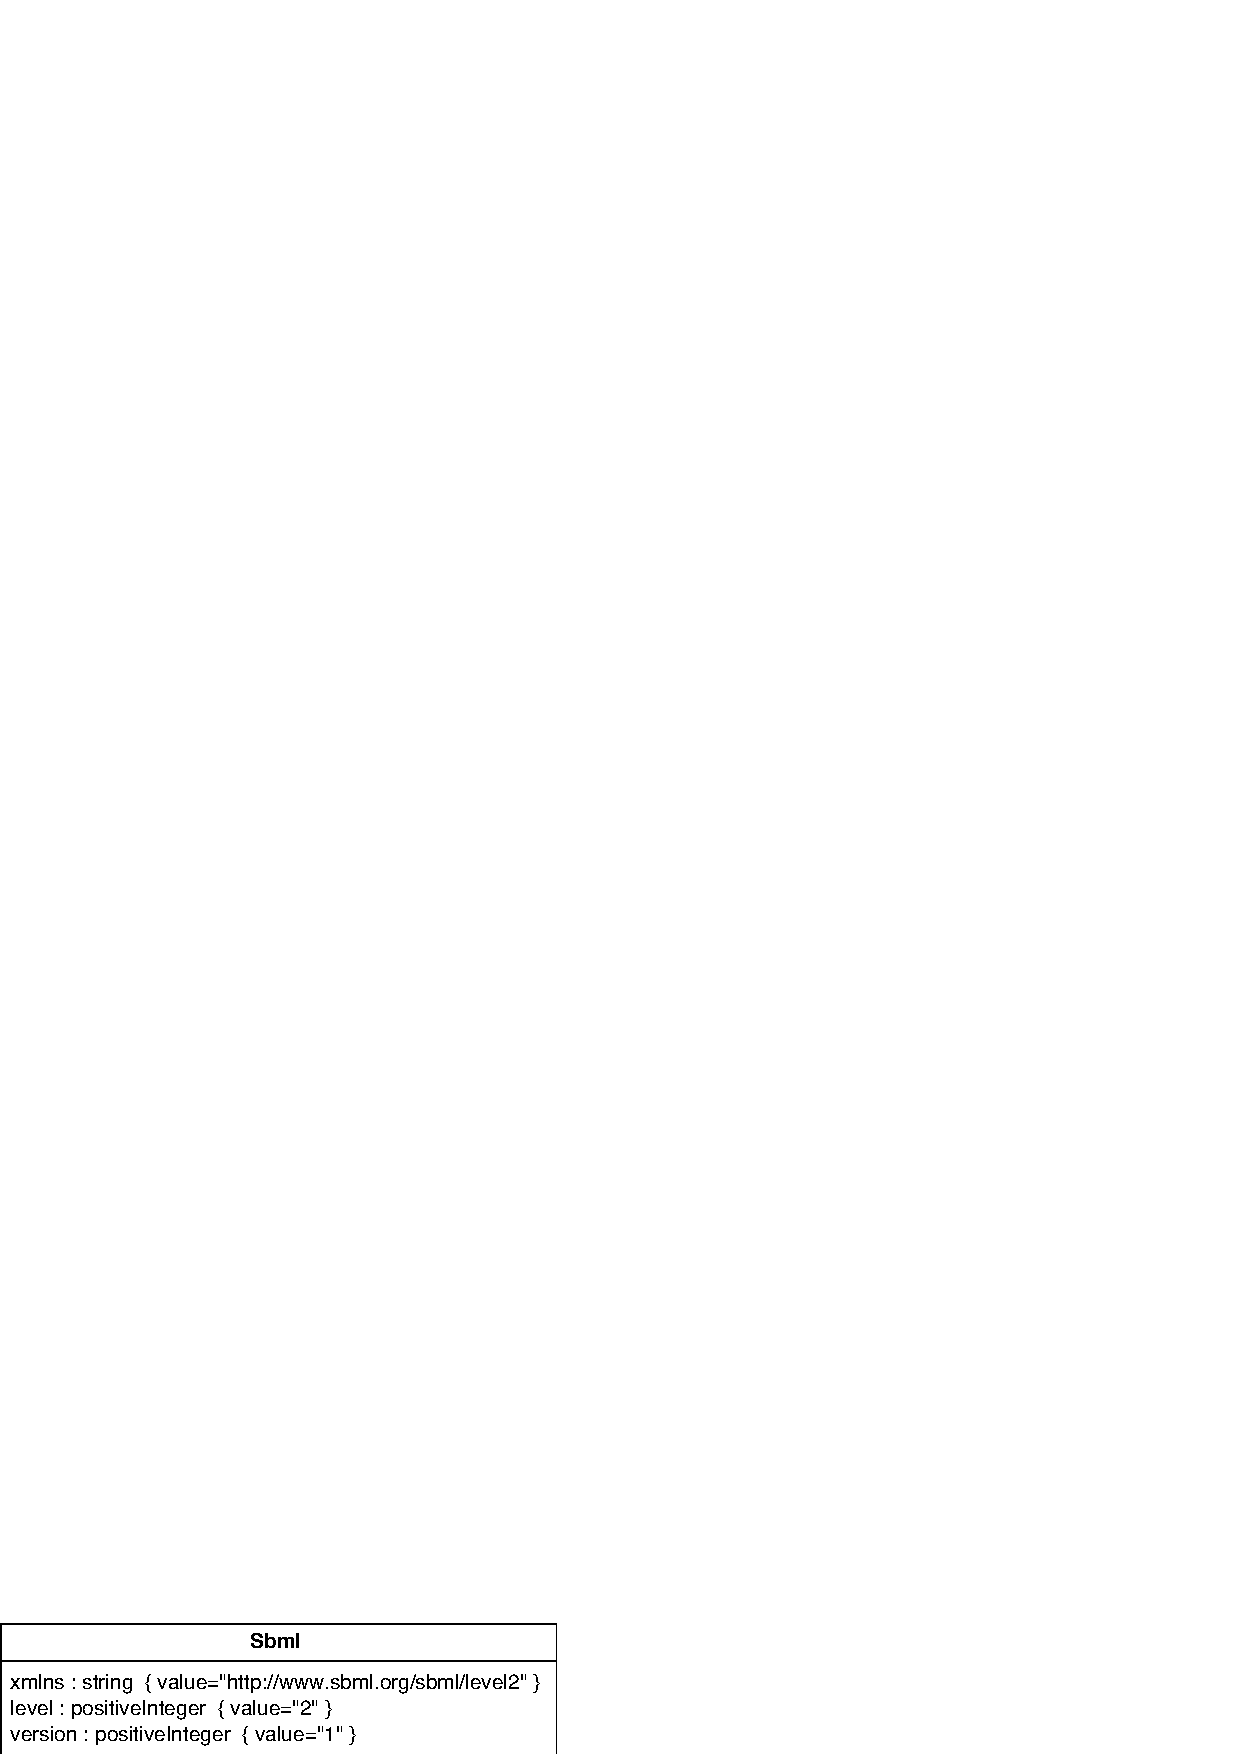
\includegraphics[scale = 0.68]{sbml}
  \caption{The definition of \class{Sbml}.  Additional fields are
    inherited from \class{SBase} but are not shown here.}
  \label{fig:sbml}
\end{figure}

The XML namespace URI for SBML Level~2 is
\texttt{http://www.sbml.org/sbml/level2}.  In the transformation of UML to
XML used in this document, the \class{Sbml} structure is turned into an
element named \texttt{sbml}.  The element has two required attributes:
\attrib{version} and \attrib{level}.  For SBML Level~2 Version~1, these
attributes must be set to ``\texttt{1}'' and ``\texttt{2}'', respectively.
(The \texttt{version} attribute is present in case SBML Level~2 must be
revised in the future to correct errors.)

The following is an abbreviated example of the outermost content of an SBML
model definition in XML:

\begin{example}
<?xml version="1.0"?>
<sbml xmlns="http://www.sbml.org/sbml/level2" version="1" level="2">
  ...
</sbml>
\end{example}


%-----------------------------------------------------------------------------
\subsection{Models}
\label{sec:model}
%-----------------------------------------------------------------------------

The \class{Model} structure is the highest-level construct in an SBML data
stream or document.  It defines a grouping of components---the list of
function definitions, compartments, species, reactions, parameters, rules
and unit definitions that define a given model.  Only one component of type
\class{Model} is allowed per instance of an SBML Level~2 document or data
stream, although it does not necessarily need to represent a single
biological entity.  The UML definition of the \class{Model} structure is
shown in Figure~\vref{fig:model}.

\begin{figure}[htb]
  \centering
  
\includegraphics[scale = 0.68]{model}
  \caption{The definition of \class{Model}.  Additional fields are
    inherited from \class{SBase}.}
  \label{fig:model}
\end{figure}

The \class{Model} structure has an optional field, \attrib{id}, used to
give the model an identifier.  The identifier must be a text string
conforming to the syntax permitted by the \class{SId} data type described
in Section~\ref{sec:id}.  \class{Model} also has an optional \attrib{name}
field, of type \class{string}.  The \attrib{name} and \attrib{id} fields
should be used as described in Section~\ref{sec:idnameattribs}.

\class{Model} serves as a container for \class{Species},
\class{Compartment}, \class{FunctionDefinition}, \class{UnitDefinition},
\class{Parameter}, \class{Reaction}, \class{Rule} and \class{Event}
components.  All of these components are optional (the lists in each of the
respective fields are permitted to have zero length).  In the XML encoding
of an SBML model, the lists of species, compartments, unit definitions,
parameters, reactions, function definitions, rules and events are
translated into lists of XML elements that each have headings of the form
\class{listOf}\rule{0.5in}{0.5pt}\class{s}, where the blank is replaced by
the name of the component type (e.g., ``\texttt{Reaction}'').  The
resulting XML data object has the form illustrated by the following
skeletal model:

\begin{example}
<model id="My_Model">
    <listOfFunctionDefinitions>
        ...
    </listOfFunctionDefintions>
    <listOfUnitDefinitions>
        ...
    </listOfUnitDefinitions>
    <listOfCompartments>
        ...
    </listOfCompartments>
    <listOfSpecies>
        ...
    </listOfSpecies>
    <listOfParameters>
        ...
    </listOfParameters>
    <listOfRules>
        ...
    </listOfRules>
    <listOfReactions>
        ...
    </listOfReactions>
    <listOfEvents>
        ...
    </listOfEvents>
</model>
\end{example}

Readers may wonder about the motivations for the
\class{listOf}\rule{0.5in}{0.5pt}\class{s} notation.  A simpler approach to
creating the lists of components would be to place them all directly
at the top level under \texttt{<model> ... </model>}.  We chose instead to
group them within XML elements named after
\class{listOf}\rule{0.5in}{0.5pt}\class{s}, because we believe this helps
organize the components and makes visual reading of model definitions
easier.

%-----------------------------------------------------------------------------
\subsection{Function Definitions}
\label{sec:functions}
%-----------------------------------------------------------------------------

The \class{FunctionDefinition} structure associates an identifier with a
function definition.  The identifier can then be used in any subsequent
MathML \class{apply} elements.  \class{FunctionDefinition} is shown in
Figure~\vref{fig:mathdefinition}.

\begin{figure}[htb]
  \vspace*{5pt}
  \centering
  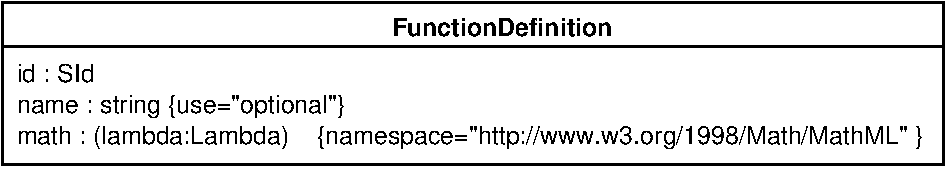
\includegraphics[scale = 0.68]{mathdefinition}
  \caption{The definition of \class{FunctionDefinition}.  Fields inherited
  from \class{SBase} are omitted here but are assumed.}
  \label{fig:mathdefinition}
\end{figure}

The \class{FunctionDefinition} structure has three fields, \attrib{id},
\attrib{name} and \attrib{math}.  The \attrib{id} and \attrib{name} fields
have types \class{SId} and \class{string}, respectively, and operate in the
manner described in Section~\ref{sec:idnameattribs}.  MathML \texttt{ci}
elements can refer to the function defined by a \class{FunctionDefinition}
using the value of its \attrib{id} field.

The \attrib{math} field is a container for MathML content that defines the
function.  The content of this field can only be a MathML \texttt{lambda}
element.  The function is only available for use in other MathML elements
that follow the place of its definition in an SBML model.  (This
restriction is to prevent recursive and mutually-recursive functions from
being expressed.)

The following is an abbreviated SBML example.  It shows a
\class{FunctionDefinition} structure defining $pow3(x)$ as representing
$x^{3}$:

\begin{example}
<model>
    ...
    <functionDefinition id="pow3">
        <math xmlns="http://www.w3.org/1998/Math/MathML">
            <lamdba>
                <bvar><ci> x </ci></bvar>
                <apply>
                    <power/>
                    <ci> x </ci>
                    <cn> 3 </cn>
                </apply>
            </lamdba>
        </math>
    </functionDefinition>
    ...
</model>
\end{example}

%-----------------------------------------------------------------------------
\subsection{Unit Definitions}
\label{sec:unitdefinitions}
%-----------------------------------------------------------------------------

Units may be supplied in a number of contexts in an SBML model.  A facility
for defining units is convenient to have so that combinations of units can
be given abbreviated names.  This is the motivation behind the
\class{UnitDefinition} data structure, whose definition is shown in
Figure~\vref{fig:unitdefinition}.

\begin{figure}[htb]
  \vspace*{8pt}
  \centering
  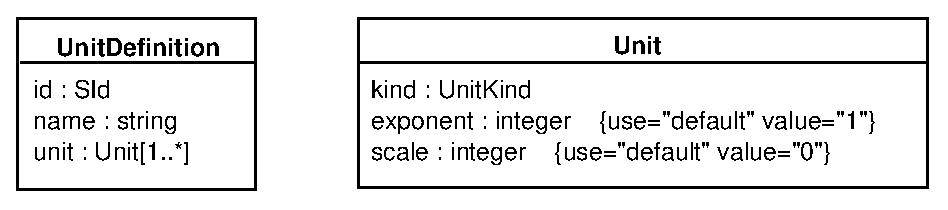
\includegraphics[scale = 0.68]{unitdefinition}
  \caption{The definition of \class{UnitDefinition}.}
  \label{fig:unitdefinition}
\end{figure}

A unit definition consists of a \attrib{id} field of type \class{SId}, an
optional string field \attrib{name} and an optional list of structures of
type \class{Unit}. The identifiers defined in the \attrib{id} field are in
a separate global namespace from identifiers for species, compartments,
reactions, events, etc.

The approach to defining units in SBML is compositional; for
example, $meter\ second^{\,-2}$ is constructed by combining a
\class{Unit}-type element representing $meter$ with a
\class{Unit}-type element representing $second^{\,-2}$.  The
\class{Unit} data structure has a required field, \attrib{kind}, whose value
must be taken from \class{UnitKind}, an enumeration of units.
The possible values of \class{UnitKind} are listed in
Table~\vref{tab:unitkind}.  The \attrib{exponent} field on
\class{Unit} represents an exponent on the unit.  Its default
value is ``\attribvalue{1}'' (one).  In the example just
mentioned, $second^{\,-2}$ is obtained by using
\texttt{kind="second"} and \texttt{exponent="-2"}. Finally, the
\attrib{scale} field in \class{Unit} is an integer attribute that
scales the unit.  For example, a unit that has a \attrib{kind}
value of ``\texttt{gram}'' and a \attrib{scale} value of
``\texttt{$-3$}'' signifies $10^{-3} * gram$, or milligrams.

\begin{table}[bh]
  \centering
  \vspace*{10pt}                        % SPECIFIC ADJUSTMENT FOR THIS PAGE
  \ttfamily
  \begin{tabular}{llllll}
    \toprule
    ampere      & farad & joule     & lumen     & ohm     & steradian\\
    becquerel   & gram  & katal     & lux       & pascal  & tesla\\
    candela & gray  & kelvin    & meter     & radian  & volt\\
    Celsius     & henry & kilogram  & metre     & second  & watt\\
    coulomb & hertz & liter     & mole      & siemens & weber\\
    \underline{dimensionless} & \underline{item} & litre    & newton    & sievert\\
    \bottomrule
  \end{tabular}
  \caption{The possible values of \attrib{kind} in a \class{UnitKind}
    structure.  All are names of base or derived SI units, except for
    ``\texttt{dimensionless}'' and ``\texttt{item}'', which are 
    SBML additions important for handling certain common cases.
    ``\texttt{Dimensionless}'' is intended for cases where a quantity does not
    have units, and ``\texttt{item}'' is  needed in certain contexts to express
    such things as ``N items'' (e.g., ``100 molecules'').
    \changed{Although ``\texttt{Celsius}'' is capitalized, for 
    simplicity, SBML
    requires that these names be treated in a case-insensitive manner.
    Also, note that the gram and liter/litre are not
    strictly part of SI~\protect\citep{bipm:2000}; however, they are so
    commonly used in SBML's areas of application that they 
    are included as predefined unit names.}  (The standard SI unit of
    mass is in fact the kilogram, and volume is
    defined in terms of cubic meters.)}
  \label{tab:unitkind}
\end{table}

Unit combinations are constructed by listing several \class{Unit}
structures inside a \class{UnitDefinition}-type structure.  The following
example illustrates the definition of an abbreviation named
``\texttt{mmls}'' for the units $mmol\ l^{-1}\ s^{-1}$:

\begin{example}
<listOfUnitDefinitions>
    <unitDefinition id="mmls">
        <listOfUnits>
            <unit kind="mole"   scale="-3"/>
            <unit kind="litre"  exponent="-1"/>
            <unit kind="second" exponent="-1"/>
        </listOfUnits>
    </unitDefinition>
</listOfUnitDefinitions>
\end{example}

There are three special unit names in SBML, listed in
Table~\ref{tab:builtin}, corresponding to the three types of quantities
that play roles in biochemical reactions: amount of substance, volume and
time.  SBML defines default units for these quantities, all with a default
\texttt{scale} value of \texttt{0}.  The various components of a model,
such as parameters, can use only the predefined units from
Table~\ref{tab:unitkind}, new units defined in unit definitions, or the
three predefined names ``\texttt{substance}'', ``\texttt{time}'', and
``\texttt{volume}'' from Table~\ref{tab:builtin}.  The latter usage
signifies that the units to be used should be the designated defaults.  

\begin{table}[htb]
  \vspace*{10pt}                        % SPECIFIC ADJUSTMENT FOR THIS PAGE
  \centering
  \small
  \setlength{\tabcolsep}{4.5pt}
  \begin{blockChanged}
  \begin{tabular}{lllc}
    \toprule
    \textbf{Name} & \textbf{Allowable Units} & \textbf{Default Units}\\
    \midrule
    \texttt{substance} & moles \emph{or} no. of molecules     & moles \\
    \texttt{volume}                & liters           & liters \\
    \texttt{time}                  & seconds          & seconds \\
    \bottomrule
  \end{tabular}
  \end{blockChanged}
  \caption{SBML's built-in quantities.  Each of these units has a default
  \texttt{scale} value of \texttt{0}.}
  \label{tab:builtin}
\end{table}

A model may change the default scales by reassigning the keywords
``\texttt{substance}'', ``\texttt{time}'', and ``\texttt{volume}'' in a
unit definition.  This takes advantage of the \class{UnitDefinition}
structure's facility for defining scales on units.  The following example
changes the default units of volume to be milliliters:

\begin{example}
<model>
    ...
    <listOfUnitDefinitions>
        <unitDefinition id="volume">
            <listOfUnits>
                <unit kind="liters" scale="-3"/>
            </listOfUnits>
        </unitDefinition>
    </listOfUnitDefinitions>
    ...
</model>
\end{example}

If the definition above appeared in a model, the volume scale on all
components that did not explicitly use different units would be changed to
milliliters.


%-----------------------------------------------------------------------------
\subsection{Compartments}
\label{sec:compartments}
%-----------------------------------------------------------------------------

A \class{Compartment} represents a bounded container in which
species are located.  The definition of \class{Compartment} is
shown in Figure~\vref{fig:compartment}.

\begin{figure}[htb]
  \centering
  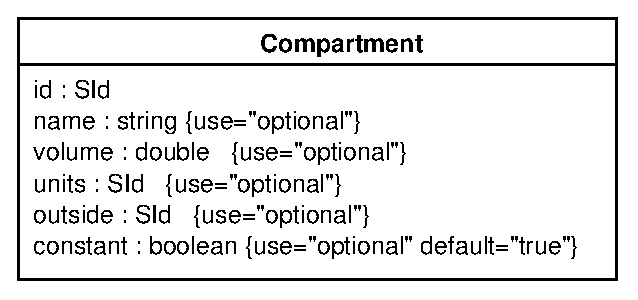
\includegraphics[scale = 0.68]{compartment}
  \caption{The definition of \class{Compartment}.
    Fields inherited from \class{SBase} are omitted here but are assumed.}
  \label{fig:compartment}
\end{figure}

A \class{Compartment} data object has an \attrib{id} field of type
\class{SId} and an optional \attrib{name} field of type
\class{string}.  A compartment also has a floating-point field
called \attrib{volume}, representing the total volume of the
compartment in the default units of volume.  (See
Table~\vref{tab:builtin}.)  This enables concentrations of species
to be calculated in the absence of geometry information. The
\attrib{volume} field is optional.  A missing \attrib{volume} value
implies that the value is either unknown, not required for analysis,
or available from an external data source.  A missing \attrib{volume}
value does not imply that the compartment volume is 1.

A \class{Compartment} structure has an optional boolean field called
\attrib{constant} which indicates whether the compartment's volume stays
constant or can vary during a simulation.  A value of \attribvalue{false}
indicates that the compartment's volume can be determined by rules, and the
value of the \attrib{volume} field should be taken to be the initial volume
of the compartment.  The default value for the \attrib{constant} field is
\attribvalue{true} because in typical modeling scenarios, compartment
volumes do not change.

The units of volume may be explicitly set using the optional field
\attrib{units} in \class{Compartment}; the named units must be either one
of the base units from Table~\vref{tab:unitkind}, the built-in default
named \attrib{volume}, or a new unit defined by a unit definition in the
enclosing model.  If absent, the units default to the value set by the
built-in \attrib{volume} of Table~\ref{tab:builtin}.

In an XML data stream containing an SBML model, compartments are listed
inside an XML element called \attrib{listOfCompartments} within a
\class{Model}-type data structure.  (See the discussion of \class{Model} in
Section~\ref{sec:model}.)  The following example illustrates two
compartments in an abbreviated SBML example of a model definition:

\begin{example}
<model>
    ...
    <listOfCompartments>
        <compartment id="cytosol" volume="2.5"/>
        <compartment id="mitochondria" volume="0.3"/>
    </listOfCompartments>
    ...
</model>
\end{example}

On the \class{Compartment} structure, the optional field \attrib{outside}
of type \class{SId} can be used to express containment relationships
between compartments.  If present, the value of \attrib{outside} for a given
compartment should be the identifier of the compartment enclosing it, or in
other words, the compartment that is ``outside'' of it.  This facility can
be used to model cell membranes.  For example, to express that a
compartment B has a membrane that is modeled as another compartment M,
which in turn is located within another compartment A, one would write:
\begin{example}
<model>
    ...
    <listOfCompartments>
        <compartment id="A"/>
        <compartment id="M" outside="A"/>
        <compartment id="B" outside="M"/>
    </listOfCompartments>
    ...
</model>
\end{example}

In the absence of a value for \attrib{outside}, compartment definitions in
SBML Level~2 do not have any implied spatial relationships between each
other.  For many modeling applications, the transfer of substances
described by the reactions in a model sufficiently express the
relationships between the compartments.  (SBML Level~2 currently does not
provide for spatial characteristics aside from compartment volume and
containment.  As discussed in Section~\ref{sec:level-3}, we expect that
SBML Level~3 will introduce the ability to define geometries and spatial
qualities.)


%-----------------------------------------------------------------------------
\subsection{Species}
\label{sec:species}
%-----------------------------------------------------------------------------

The term \emph{species} refers to chemical entities that take part in
reactions.  These include simple ions (e.g., protons, calcium), simple
molecules (e.g., glucose, ATP), and large molecules (e.g., RNA,
polysaccharides, and proteins).  The \class{Species} data structure is
intended to represent these entities.  Its definition is shown in
Figure~\vref{fig:species}.

\begin{figure}[htb]
  \vspace*{8pt}
  \centering
  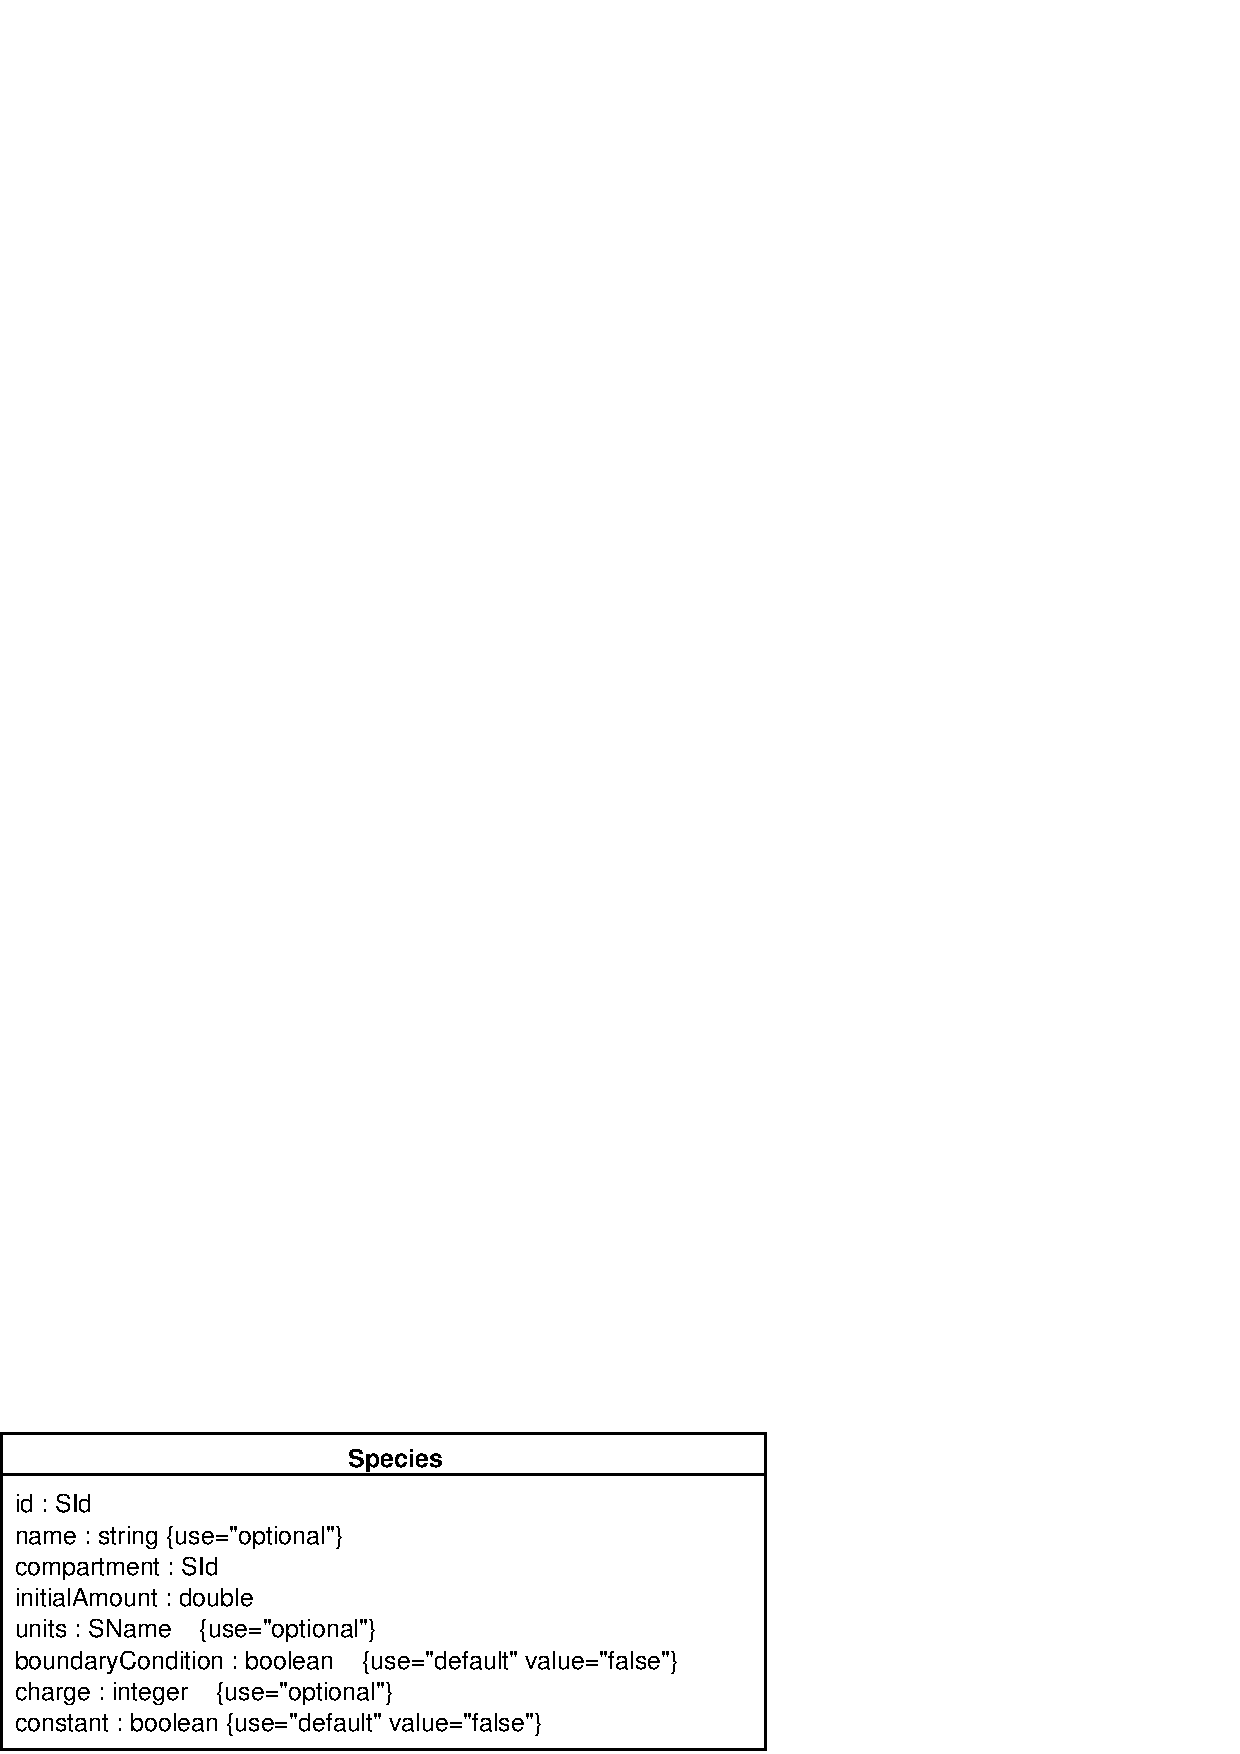
\includegraphics[scale = 0.68]{specie}
  \caption{The definition of \class{Species}.  As usual, fields inherited from
    \class{SBase} are omitted here but are assumed.}
  \label{fig:species}
\end{figure}

\class{Species} has an \attrib{id} field of type \class{SId} and optional
\attrib{name} field of type \class{string}.  The field
\attrib{compartment}, also of type \class{SId}, is used to identify the
compartment in which the species is located.  The optional field
\attrib{initialAmount}, of type \class{double}, is used to set the initial
amount of the species in the named compartment.  A missing \attrib{initialAmount} value
implies that the value is either unknown, not required for analysis
or available from an external data source.  The units of the substance
quantity may be explicitly set using the optional field \attrib{units}.  The
value assigned to \attrib{units} must be chosen from one of the following
possibilities: one of the unit names from Table~\vref{tab:unitkind}, the
name ``\attrib{substance}'', or a new unit name defined by a unit
definition in the enclosing model.  If absent, the units default to the
value set by the built-in ``\attrib{substance}'' of
Table~\vref{tab:builtin}.

The \class{Species} structure has an optional boolean field named
\attrib{constant} which indicates whether the concentration of that species
can vary during a simulation.  The default value is \attribvalue{false},
indicating that the species' concentration can be determined by rules and
reactions.

\class{Species} also has another optional boolean field,
\attrib{boundaryCondition}.  By default, when a species is a product or
reactant of one or more reactions, the concentration of that species is
determined by those reactions.  In SBML, it is possible to indicate that a
given species' concentration is \emph{not} determined by the set of
reactions even when that species occurs as a product or reactant; i.e., the
species is on the \emph{boundary} of the reaction system but is a component
of the rest of the model.  The optional boolean field
\attrib{boundaryCondition} indicates that the given species is on the
boundary of the reaction system.  The value of the field defaults to
``\attribvalue{false}'', indicating that by default, the species \emph{is}
part of the reaction system.  Table~\ref{tab:specieattrib} shows how to
interpret the combined values of the \attrib{boundaryCondition} and
\attrib{constant} fields.  In practice, the \attrib{boundaryCondition}
attribute means that a differential equation derived from the reaction
definitions should not be generated for the species.  The example model in
section~\ref{sec:constantspecieseg} contains all 4 possible states of the
\attrib{boundaryCondition} and \attrib{constant} attributes on
\class{species} elements.

\begin{table}[ht]
  \vspace*{10pt}
  \centering
  \begin{tabular}{lllll}
    \toprule
    \textbf{\attrib{constant}} & \textbf{\attrib{boundaryCondition}} &
    \textbf{can have} & \textbf{can be} & \textbf{concentration} \\
    \textbf{value} & \textbf{value} & \textbf{assignment} & \textbf{reactant or} & \textbf{is changed by} \\
    & & \textbf{rule} & \textbf{product}\\
    \midrule
    true & true & no & yes & never changes\\
    false & true & yes & yes & rule \\
    true & false & no & no & never changes \\
    false & false & yes & yes & reactions or rule but not both \\
    \bottomrule
  \end{tabular}
  \caption{How to interpret the values of the \attrib{constant} and
    \attrib{boundaryCondition} fields of the \class{Species} structure.}
  \label{tab:specieattrib}
\end{table}

The optional field \attrib{charge} on \class{Species} takes an integer
indicating the charge on the species (in terms of electrons, not the SI
unit Coulombs). This may be useful when the species involved is a charged
ion such as calcium ($\text{Ca}^{2+}$).

The following example shows two species definitions within an
abbreviated SBML model definition.  The example shows that species
are listed under the heading \attrib{listOfSpecies} in the model:

\begin{example}
<model>
    ...
    <listOfSpecies>
        <species id="Glucose" compartment="cell" initialAmount="4"/>
        <species id="Glucose_6_P" compartment="cell" initialAmount="0.75"/>
    </listOfSpecies>
    ...
</model>

\end{example}

\vspace*{5pt}                           % ADJUSTMENT FOR THIS PAGE ONLY.

%-----------------------------------------------------------------------------
\subsection{Parameters}
\label{sec:parameters}
%-----------------------------------------------------------------------------

A \class{Parameter} structure is used to declare a variable for use in
mathematical formulas in an SBML model definition.  By default, parameters
have constant value for the duration of a simulation and are therefore
called ``parameters'' instead of variables in SBML.  The definition of
\class{Parameter} is shown in Figure~\vref{fig:parameter}.

\begin{figure}[htb]
  \vspace*{12pt}                           % ADJUSTMENT FOR THIS PAGE ONLY.
  \centering
  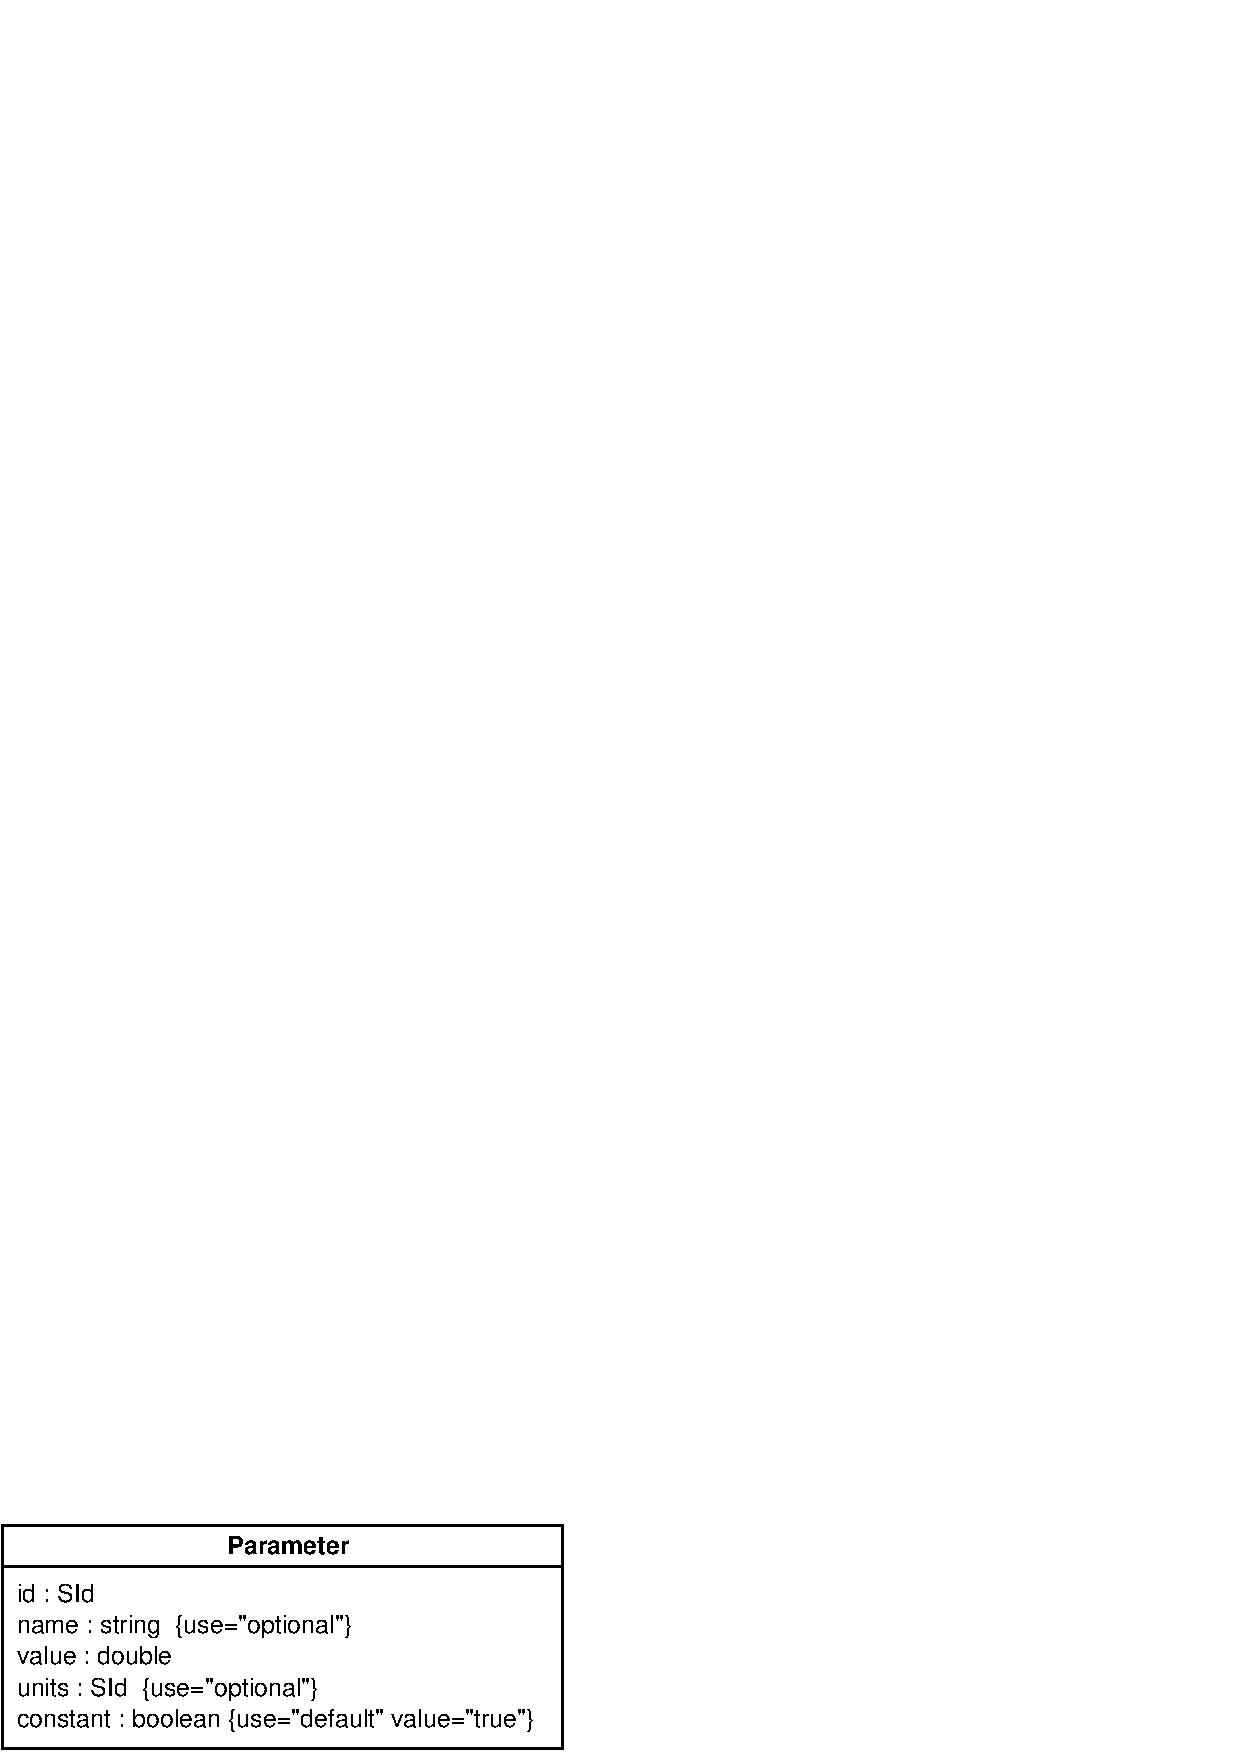
\includegraphics[scale = 0.68]{parameter}
  \caption{The definition of \class{Parameter}.   Fields inherited from
    \class{SBase} are omitted here but are assumed.}
  \label{fig:parameter}
\end{figure}

\class{Parameter} has an \attrib{id} field of type \class{SId} and
an optional \attrib{name} field of type \class{string}.  The
symbol in the \attrib{id} field identifies the parameter.  The
optional field \attrib{value} determines the value (of type \class{double})
assigned to the identifer.  A missing \attrib{value} 
implies that the \attrib{value} is either unknown, not required for analysis
or available from an external data source.  The units of the parameter
\attrib{value} are specified by the optional field \attrib{units}.
The value assigned to \attrib{units} must be chosen from one of
the following possibilities: one of base unit names from
Table~\vref{tab:unitkind}; one of the three names
``\attribvalue{substance}'', ``\attribvalue{time}'', or
``\attrib{volume}'' (see Table~\ref{tab:builtin}); or the name of
a new unit defined in the list of unit definitions in the
enclosing \class{Model} structure.

The \class{Parameter} structure has an optional boolean field named
\attrib{constant} which indicates whether the parameter's value can vary
during the simulation.  The default value is \attribvalue{true}; a value of
\attribvalue{false} indicates that the parameter's value can be changed by
rules (see Section~\ref{sec:rules}) and that the \attrib{value} is actually
intended to be the initial value of the parameter.

Parameters are used in two places in SBML: in lists of parameters defined
at the top level in a \class{Model}-type structure, and within individual
reaction definitions.  Parameters defined at the top level are
\emph{global} to the whole model; parameters that are defined within
a reaction are local to the particular reaction and (within that reaction)
\emph{override} any global parameters having the same names.  (See
Section~\ref{sec:namespaces} for further details.)

The following is an example of parameters defined at the \class{Model} level:

\begin{example}
<model>
    ...
    <listOfParameters>
        <parameter id="Km1" value="2.3" units="second"/>
        <parameter id="Km2" value="10.7" units="second"/>
    </listOfParameters>
    ...
</model>
\end{example}

%-----------------------------------------------------------------------------
\subsection{Rules}
\label{sec:rules}
%-----------------------------------------------------------------------------

In SBML, \emph{rules} provide a way to create constraints on variables for
cases in which the constraints cannot be expressed using the reaction
components (Section~\ref{sec:reactions}). There are three different
possible functional forms of rules, corresponding to the following three
general cases (where $x$ is a variable, $f$ is some arbitrary function, and
$X$ is the vector of variables that may include species, compartments and
parameters):

\begin{center}
\begin{tabular}{ll}
  \emph{Algebraic} rules, left-hand side is zero:             & $0 = f(X)$\\
  \emph{Scalar} rules, left-hand side is a scalar:         & $x = f(X)$\\
  \emph{Rate} rules, left-hand side is a rate-of-change: & $dx/dt = f(X)$
\end{tabular}
\end{center}

In their general form given above, there is little to distinguish between
\emph{scalar} and \emph{algebraic} rules.  They are treated as separate
cases for the following reasons:
\begin{itemize}
  
\item \emph{Scalar} rules can simply be evaluated to calculate intermediate
  values for use in numerical methods;
  
\item Some simulators do not contain numerical solvers capable of solving
  unconstrained \emph{algebraic} equations;
  
\item Those simulators that \emph{can} solve these \emph{algebraic}
  equations make a distinction between the different categories listed
  above; and
  
\item Some specialized numerical analyses of models may only be applicable to
  models that do not contain \emph{algebraic} rules.
\end{itemize}

In SBML, \emph{scalar} and \emph{rate} rules are collectively referred to
as \emph{assignment} rules.  SBML uses an abstract \class{Rule} structure
that contains only one field, \attrib{math}, to hold the right-hand side
expression, then derives subtypes of \class{Rule} that add fields to
distinguish the case of algebraic, scalar and rate rules.
Figure~\vref{fig:rules} gives the definitions of \class{Rule} and the
subtypes derived from it.  The figure shows there are two subtypes,
\class{AlgebraicRule} and \class{AssignmentRule}, defined directly from
\class{Rule}.

\begin{figure}[htb]
  \centering
  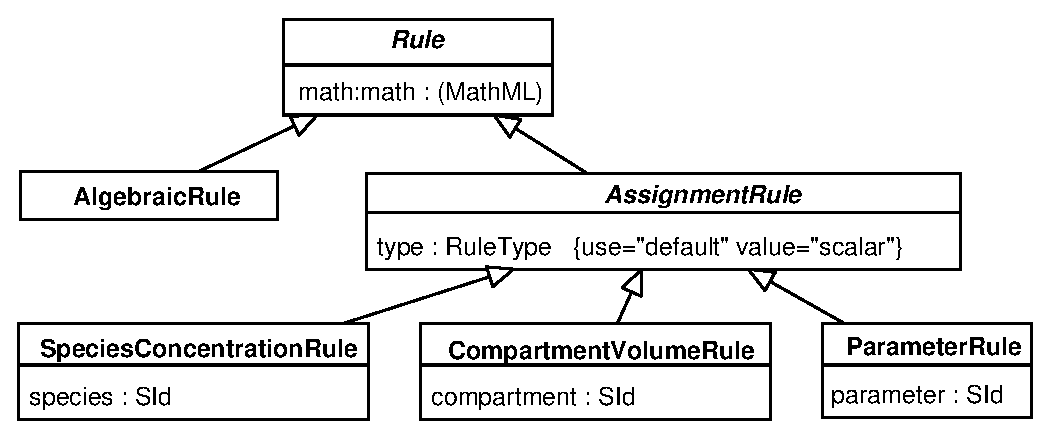
\includegraphics[scale = 0.68]{rule}
  \caption{The definition of \class{Rule} and derived types.}
  \label{fig:rules}
\end{figure}

The \attrib{type} field introduced in \class{AssignmentRule} is an
enumeration of type \class{RuleType} that determines whether a
rule falls into the \emph{scalar} or \emph{rate} categories. In
SBML Level~2, the enumeration has two possible values:
``\class{scalar}'' and ``\class{rate}''.  The former means that
the expression has a scalar value on the left-hand side [i.e., $x
= f(X)$]; the latter means that
the expression has a rate of change differential on the left-hand
side [i.e. $dx/dt = f(X)$]. Future releases of SBML may
add to the possible values of \class{RuleType}.


\subsubsection{\class{AlgebraicRule}}

The rule type \class{AlgebraicRule} is used to express equations whose
left-hand sides are zero.  \class{AlgebraicRule} does not add any fields to
the basic \class{Rule}; its role is simply to distinguish this case from
the assignment rule case.  An example of the use of \class{AlgebraicRule}
structures is given in Section~\ref{sec:algeraiceg}.

\subsubsection{\class{AssignmentRule}}

The left-hand sides of assignment rules can be the identifiers of species,
compartments, or parameters.  The effects are in general terms the same,
but have different effects depending on what variable is being set:

\begin{itemize}
  
\item \emph{In the case of a species}: if the value of \attrib{type} is
  ``\class{scalar}'', the rule sets the referenced species's concentration
  to the value determined by the formula in \attrib{math}; if the value is
  ``\class{rate}'', the rule sets the rate of change of the species's
  concentration to the value determined by the formula.  The units are in
  terms of $substance/volume$, where the $substance$ units are those that
  are declared on the referenced \class{Species} element, and the $volume$
  units are those declared on the \class{compartment} element that contains
  the \class{Species}.
  
  \emph{Restrictions}: A rule and a \class{SpeciesReference} structure (see
  Section~\ref{sec:reactions}) cannot both have the same \attrib{species}
  attribute value.  This means that a rule cannot be defined for a species
  that is created or destroyed in a reaction.  The only exception is when
  the given species is a boundary condition; i.e., on the \class{Species}
  structure that defines the specie the \attrib{boundaryCondition} field is
  set to ``\attribvalue{true}''.
  
\item \emph{In the case of a compartment}: if the value of \attrib{type} is
  ``\class{scalar}'', the rule sets the referenced compartment's volume to
  the volume determined by the formula in \attrib{math}; if the type is
  ``\class{rate}'', the rule sets the rate of change of the compartment's
  volume to the volume determined by the formula.
  
  \emph{Restrictions}: No more than one \class{AssignmentRule} can refer to
  a given compartment in an SBML model definition.
  
\item \emph{In the case of a parameter}: if the value of \attrib{type} is
  ``\texttt{scalar}'', the rule sets the referenced parameter's value to
  that determined by the formula in \attrib{math}; if the type is
  ``\texttt{rate}'', the rule sets the rate of change of the parameter's
  value to that determined by the formula.
  
  \emph{Restrictions}: No more than one \class{AssignmentRule} can refer to
  a given parameter.

\end{itemize}

\subsubsection{Constraints on rules}
\label{sec:ruleconstraints}

SBML specifically does not stipulate the form of the algorithms that can be
applied to rules and reactions.  For example, SBML does not specify when or
how often rules should be evaluated.  The constraints described by rules
and kinetic rate laws are meant to apply collectively to the set of
variable values for a specific time.

In SBML, no more than one assignment rule can be defined for a given
identifier.  No assignment rule can be defined for an identifier whose
corresponding structure has the field \attrib{constant} set to
\attribvalue{true}.

A \texttt{scalar} rule for a given identifier overrides the initial value
of that identifier; i.e., the initial value should be ignored.  This does
not mean that any structure declaring an identifier can be omitted if there
is a \texttt{scalar} rule for that identifier.  For example, there must be
a \texttt{Parameter} structure for a given parameter if there is a rule for
that parameter.

The ordering of \texttt{scalar} rules is significant: they are always
evaluated in the order given in SBML.  The \attrib{math} field of a
\texttt{scalar} rule structure can contain any identifier in a MathML
\class{ci} element except for the following: (a) identifiers for which
there exists a subsequent \texttt{scalar} rule, and (b) the identifier for
which the rule is defined.  These constraints are designed to eliminate
algebraic loops among the scalar rules.  As an example, consider the
following equations, in the order shown:
\begin{equation*}
  \begin{array}{lll}
    x = x + 1, & y = z + 200, & z = y + 100
  \end{array}
\end{equation*}
If this set of equations were interpreted as a set of scalar rules, it
would be invalid because the rule for $x$ refers to $x$ and the rule for
$y$ refers to $z$ before $z$ is defined.

Eliminating these algebraic loops ensures that scalar rules can be
evaluated any number of times without the result of those
evaluations changing.


\subsubsection{Example of Rule Use}
\label{sec:eg-rule-use}

This section contains an example set of rules.  Consider the following
set of equations:
\begin{equation*}
  \begin{array}{lll}
    k = \D\frac{k_3}{k_2}, & s_2 = \D\frac{k t}{1 + k_2}, & A = 0.10 t
  \end{array}
\end{equation*}
This math can be encoded by the following scalar rule set:
\begin{example}
<model>
    ...
    <listOfRules>
        <assignmentRule id="k">
            <notes>
                <xhtml:p>
                    k = k3/k2
                </xhtml:p>
            </notes>
            <math xmlns="http://www.w3.org/1998/Math/MathML">
                <apply>
                    <divide/>
                    <ci> k3 </ci>
                    <ci> k2 </ci>
                </apply>
            </math>
        </assignmentRule>
        <assignmentRule variable="s2">
            <notes>
                <xhtml:p>
                    s2 = (k * t)/(1 + k2)
                </xhtml:p>
            </notes>
            <math xmlns="http://www.w3.org/1998/Math/MathML">
                <apply>
                    <divide/>
                    <apply>
                        <times/>
                        <ci> k </ci>
                        <ci> t </ci>
                    </apply>
                    <apply>
                        <plus/>
                        <cn> 1 </cn>
                        <ci> k2 </ci>
                    </apply>
                </apply>
            </math>
        </assignmentRule>
        <assignmentRule variable="A">
            <notes>
                <xhtml:p>
                    A = 0.10 * t
                </xhtml:p>
            </notes>
            <math xmlns="http://www.w3.org/1998/Math/MathML">
                <apply>
                    <times/>
                    <cn> 0.10 </cn>
                    <ci> t </ci>
                </apply>
            </math>
        </assignmentRule>
    </listOfRules>
    ...
</model>
\end{example}


%\subsubsection{Guidelines for Evaluating Rules}
%
%This section describes how rules including those implied by
%\class{Reaction} structures (see Section~\ref{sec:reactions})
%should be evaluated.  For the purpose of interpreting models
%mathematically (and for this description), \class{Reaction}
%structures collectively imply a \class{SpeciesConcentrationRule}
%structure, of type \class{rate}, for each species referenced in a
%\class{SpeciesReference} structure excluding those species which
%are defined with the \attrib{boundaryCondition} attribute equal to
%\texttt{true}.
%
%To determine the initial values of variables is a 2 set process:
%
%\begin{itemize}
%
%\item variables should be set according to the initial values
%given by \class{Species}, \class{Compartment} and
%\class{Parameter} structures then
%
%\item the \class{scalar} rules should be evaluated
%
%\end{itemize}
%
%To determine the rates of change of variables given a set of
%current variable values is again a two set process:
%
%\begin{itemize}
%
%\item the \class{scalar} rules should be evaluated then
%
%\item the \class{rate} rules should be evaluated
%
%\end{itemize}
%
%The \class{scalar} rules should be evaluated to determine the
%complete set of variable values given an incomplete set of
%variable values determined by \class{rate} and
%\class{AlgebraicRule} structures.
%

%-----------------------------------------------------------------------------
\subsection{Reactions}
\label{sec:reactions}
%-----------------------------------------------------------------------------

A \emph{reaction} represents any transformation, transport or binding
process, typically a chemical reaction, that can transform or change the
amount of one or more species.  In SBML, a reaction is defined primarily in
terms of the participating reactants and products (and their corresponding
stoichiometries), along with optional modifier species, an optional kinetic
law describing the rate at which the reaction takes place, and optional
parameters entering into the kinetic law.  These various parts of a
reaction are recorded in the SBML \class{Reaction} type defined in
Figure~\vref{fig:reaction}.

\begin{figure}[htb]
  \centering
  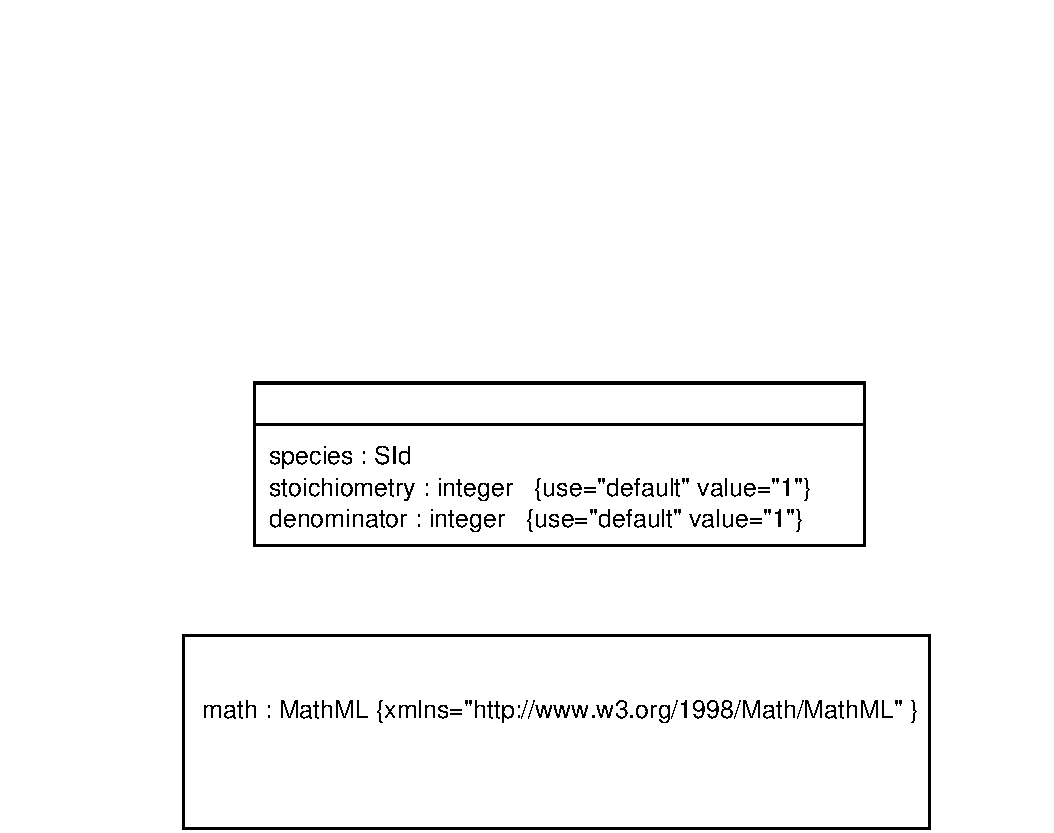
\includegraphics[scale=0.68]{reaction}
  \caption{The definitions of \class{Reaction}, \class{KineticLaw},
    \class{SpeciesReference} and \class{ModiferSpeciesReference}.}
  \label{fig:reaction}
\end{figure}

As with the other main structures in SBML, the \class{Reaction} data
structure includes a required \attrib{id} field and an optional
\class{name}.  These must be used according to the guidelines described in
Section~\ref{sec:idnameattribs}.  The reactant species, product species and
modifier species in a reaction are described using the fields
\attrib{reactant}, \attrib{product} and \attrib{modifiers}.  These fields
are optional lists of either \class{SpeciesReference} or
\class{ModifierSpeciesReference} structures, as shown in
Figure~\vref{fig:reaction}.  They are described in more detail in
Sections~\ref{subsec:speciesreference} and~\ref{subsec:modifierreference}
below.  The \attrib{kineticLaw} is an optional field of type
\class{KineticLaw}, described in more detail in
Section~\ref{subsec:kinetic-law} below.

In addition to the above, the \class{Reaction} structure also has two
optional boolean fields.  The first field, \attrib{reversible}, indicates
whether the reaction is reversible.  The field is optional, and if left
unspecified in a model, it defaults to a value of ``\attribvalue{true}''.
Although the reversibility of a reaction is determined by the rate law, the
need to allow rate laws to be optional leads to the need for a flag
indicating reversibility.  Information about reversibility in the absence
of a kinetic laws is useful in certain kinds of structural analyses such as
elementary mode analysis.  It is true that the presence of this information
in two places (i.e., the rate law and the flag \attrib{reversible}) leaves
open the possibility of a model containing contradictory information, but
the creation of such a model would indicate an error on the part of the
software generating it.  Software developers must take care to ensure
against logical contradictions in the definitions of reactions.

The field \attrib{fast} is another boolean attribute in the
\class{Reaction} data structure; a value of ``\attribvalue{true}''
signifies that the given reaction is a ``fast'' one.  This may be relevant
when computing equilibrium concentrations of rapidly equilibrating
reactions.  Simulation/analysis packages may chose to use this information
to reduce the number of ODEs required and thereby optimize such
computations.  The default value of \attrib{fast} is
``\attribvalue{false}''.  (A simulator/analysis package that has no
facilities for dealing with fast reactions can ignore this attribute. In
theory, if the choice of which reactions are fast is correctly made, then a
simulation performed with them should give the same results as a simulation
performed without fast reactions.  However, currently there appears to be
no single unambiguous method for designating which reactions should be
considered fast, and some users may designate a reaction as fast when in
fact it is not.)

\subsubsection{\class{SpeciesReference}}
\label{subsec:speciesreference}

Every species that enters into a given reaction must appear in that
reaction's lists of reactants, products or modifiers.  In an SBML model,
all species that participate in any reaction are listed in the
\attrib{listOfSpecies} field of the top-level \class{Model} data structure
(see Section~\ref{sec:model}).  Lists of products, reactants and modifiers
in \class{Reaction} type structures do not introduce new species, but
rather, they refer back to those listed in the model's
\attrib{listOfSpecies}.  For reactants and products, the connection is
made using the \class{SpeciesReference} type data structure defined
in Figure~\vref{fig:reaction}.

In \class{SpeciesReference}, the field \attrib{species} of type \class{SId}
must refer to the name of an existing species defined in the enclosing
\class{Model}-type structure.  Stoichiometric numbers for the products and
reactants can be specified using two optional attributes on the
\attrib{speciesReference} element: \attrib{stoichiometry} and
\attrib{denominator}.  Both attributes take positive integers as values,
and both have default values of ``\class{1}'' (one).  The absolute value of
the stoichiometric number is the value of \attrib{stoichiometry} divided by
\attrib{denominator}, and the sign is implicit from the role of the species
(i.e., negative for reactants and positive for products).  The use of
separate numerator and denominator terms allows a simulator to employ
rational arithmetic if it is capable of it, potentially reducing round-off
errors and other problems during computations.

The following is a simple example of a species reference in a list
of reactants within a reaction named ``J1'':
\begin{example}
<model>
    ...
    <listOfReactions>
        <reaction id="J1">
            <listOfReactants>
                <speciesReference species="X0" stoichiometry="2"/>
            </listOfReactants>
            ...
        </reaction>
        ...
    </listOfReactions>
    ...
</model>
\end{example}

A reaction can contain an empty list of reactants or an empty list of
products but must have at least one reactant or product.  Also note that
whether a given species is allowed to appear as a reactant or product is
dictated by certain flags on the structure describing the species in the
\class{Model}; see Table~\ref{tab:specieattrib} for more information.


\subsubsection{\class{ModifierSpeciesReference}}
\label{subsec:modifierreference}

In some cases, a species may act as a catalyst or inhibitor of a reaction,
and may not appear in the list of reactants or products because it is
neither created nor destroyed in that particular reaction.  In that case,
the species is known as a \emph{modifier}.  (That same species may still be
a reactant or product of another reaction.)

The \class{Reaction} structure provides a way to express which species act
as modifiers in a given reaction.  This is the purpose of the
\attrib{modifier} field in \class{Reaction}; this field is a list of
\class{ModifierSpeciesReference} structures defined in
Figure~\vref{fig:reaction}.  The \class{ModifierSpeciesReference} structure
has only one field, \attrib{species}, of type \class{SId}; its value must
be the identifier of a species defined in the enclosing \class{Model}.

The following is a simple example of a modifier species reference in a list
of reactants within a reaction named ``J1'':
\begin{example}
<model>
    ...
    <listOfReactions>
        <reaction id="J1">
            ...
            <listOfModifiers>
                <modifierSpeciesReference species="X0"/>
            </listOfModifiers>
            ...
        </reaction>
        ...
    </listOfReactions>
    ...
</model>
\end{example}

\subsubsection{\class{KineticLaw}}
\label{subsec:kinetic-law}

A \class{kineticLaw} structure describes the rate at which the reaction
takes place.  The inclusion of a \class{KineticLaw} structure in an
instance of a \class{Reaction} component is optional; however, in general
there is no useful default that can be substituted in place of a missing
rate law definition in a reaction.

The field \attrib{math} is a MathML element and contains an expression that
sets the rate of the reaction, in $substance/time$ units.
(Section~\ref{sec:formulas} discusses the use of MathML in SBML Level~2).
The optional fields \attrib{substanceUnits} and \attrib{timeUnits}
determine the units of substance and time.  If not set, the units are taken
from the defaults defined by the built-in ``\texttt{substance}'' and
``\texttt{time}'' of Table~\vref{tab:builtin}.  The only species
identifiers that can be used in \attrib{math} are those listed in the
\attrib{reactant}, \attrib{product} and \attrib{modifier} fields of the
\class{Reaction} structure.

An instance of a \class{KineticLaw} type structure can contain zero or more
\class{parameter} structures (Section~\ref{sec:parameters}) that define
symbols that can be used in the \attrib{math} element.  As discussed in
Section~\ref{sec:namespaces}, reactions introduce local namespaces for
parameter identifiers.  Within a \class{KineticLaw} structure inside a
reaction definition, a local parameter whose identifier is identical to a
global parameter defined in the enclosing \class{Model}-type structure
takes precedence over that global parameter.

The following is an example of a complete \class{Reaction} structure that
defines a reaction named $J_1$, in which $X_0 \longrightarrow S_1$ at a
rate given by $k_1 X_0 S_2$, and in which $S_2$ is a catalyst and $k_1$ is
a parameter.  It demonstrates the use of species references and the
\class{KineticLaw} structure:
\begin{example}
<model>
    ...
    <listOfReactions>
        <reaction id="J1">
            <listOfReactants>
                <speciesReference species="X0" stoichiometry="1"/>
            </listOfReactants>
            <listOfProducts>
                <speciesReference species="S1" stoichiometry="1"/>
            </listOfProducts>
            <listOfModifiers>
                <modifierSpeciesReference species="S2"/>
            </listOfModifiers>
            <kineticLaw>
                <math xmlns="http://www.w3.org/1998/Math/MathML">
                    <apply>
                        <times/>
                        <ci> k1 </ci>
                        <ci> X0 </ci>
                        <ci> S2 </ci>
                    </apply>
                </math>
                <listOfParameters>
                    <parameter id="k1" value="0.1"/>
                </listOfParameters>
            </kineticLaw>
        </reaction>
    </listOfReactions>
    ...
</model>
\end{example}


%-----------------------------------------------------------------------------
\subsection{Events}
\label{sec:events}
%-----------------------------------------------------------------------------

\class{Model} has an optional list of
\class{Event} structures that describe the time and form of explicit
instantaneous discontinuous state changes in the model.  For example, an
event may describe that one species concentration is halved when another
species concentration exceeds a given threshold value.

An \class{Event} structure defines when the event can occur, the variables
that are affected by the event, and how the variables are affected.  The
effect of the event can optionally be delayed after the occurrence of the
condition which invokes it.  The operation of an \class{Event} structure is
divided into two phases (even when the event is not delayed): one when the
event is \emph{fired} and the other when the event is \emph{executed}. The
\class{Event} type is defined in Figure~\vref{fig:event}.  Both
\class{Event} and \class{EventAssignment} are derived from \class{SBase}
(see Section~\ref{sec:sbase}).  An example of a model which uses events is
given below.

\begin{figure}[htb]
  \centering
  
\includegraphics[scale = 0.68]{event}
  \caption{The definitions of \class{Event} and \class{EventAssignment}}
  \label{fig:event}
\end{figure}

The following sections describe the fields of the \class{Event}
structure.

\subsubsection{\attrib{trigger}}
The \attrib{trigger} field defines when the \class{Event}
structure has an effect on the model.  The \attrib{trigger} field
contains a MathML boolean expression.  The exact instant that the
expression evaluates to true is the time point when the
\class{Event} is \emph{fired}.  The event only fires when the
\attrib{trigger} makes the transition from false to true.  The
event will fire at any further time points when the
\attrib{trigger} make this transition.

\subsubsection{\attrib{delay}}
The optional \attrib{delay} field defines the length of time after
the event has \emph{fired} that the event is \emph{executed}. The
\attrib{delay} field is another MathML expression.  This
expression should be evaluated when the rule is \emph{fired}.  The
default value for the \attrib{delay} field is 0.  The value of the
\attrib{delay} field should always be positive.

\subsubsection{\attrib{timeUnits}}
The optional field \attrib{timeUnits} determines the units of time
that apply to the \attrib{delay} field. If not set, the units are
taken from the defaults defined by the built-in ``\texttt{time}''
of Table~\vref{tab:builtin}.

\subsubsection{\attrib{eventAssignment}}
The \attrib{eventAssignment} field consists of a non-empty list of
\class{eventAssignment} structures.  This field is implemented as a
\class{listOfEventAssignments} element containing one or more
\class{eventAssignment} elements.  The \class{EventAssignment}
structures represent variable assignments which have effect when
the event is \emph{executed}. The \class{Assignment} structure is
shown in Figure~\ref{fig:event}. The \attrib{variable} field is of
type \class{SId} and contains the identifier of a variable i.e. a
compartment, species or parameter.  The structures referenced by
the \attrib{variable} field must have their \attrib{constant}
fields set to ``\texttt{false}''.  The \attrib{math} field
contains a MathML expression which defines the new value of the
variable.  This expression is evaluated when the \class{Event} is
\emph{fired} but the variable only acquires the result or new
value when the \class{Event} is \emph{executed}.  The order of the
\class{EventAssignment} structures is not significant (unlike
scalar rules), the effect of one assignment cannot affect the
result of another assignment.  The identifiers occurring in the
MathML \attrib{ci} fields of the \class{EventAssignment}
structures represent the value of the identifier at the point when
the \class{Event} is \emph{fired}.

A example of an \class{Event} structure follows.  This structure makes the
assignment $k_2 = 0$ at the point when $P_1 \leq t$:

\begin{example}
<event>
    <trigger>
        <math xmlns="http://www.w3.org/1998/Math/MathML">
            <apply>
                <leq/>
                <ci> P1 </ci>
                <ci> t </ci>
            </apply>
        </math>
    </trigger>
    <listOfEventAssignments>
        <eventAssignment variable="k2">
            <math xmlns="http://www.w3.org/1998/Math/MathML">
                <cn> 0 </cn>
            </math>
        </eventAssignment>
    <listOfEventAssignments>
</event>
\end{example}

A complete example model that uses events is given in Section~\ref{sec:eventeg}


%=============================================================================
\section{Example Models Expressed in XML Using SBML}
\label{sec:xml-rep}
%=============================================================================

In this section, we present several examples of complete models
encoded in XML using SBML Level~2.  

%Our approach to translating
%the UML-based structure definitions presented in the previous
%sections is described elsewhere~\citep{hucka:2000b}.
%Appendix~\ref{apdx:schemas} gives the full listing of an XML
%Schema corresponding to SBML Level~2.


%-----------------------------------------------------------------------------
\subsection{A Simple Example Application of SBML}
\label{sec:modeleg}
%-----------------------------------------------------------------------------

Consider the following hypothetical branched system:
\begin{equation*}
  \begin{array}{@{}ccc@{}}
    X_0 & \underrightarrow{k_1 X_0} & S_1 \\ \\[-4pt]
    S_1 & \underrightarrow{k_2 S_1} & X_1 \\ \\[-4pt]
    S_1 & \underrightarrow{k_3 S_1} & X_2
  \end{array}
\end{equation*}

The following is an XML document that encodes the model shown
above:

\begin{example}
<?xml version="1.0"?>
<sbml xmlns="http://www.sbml.org/sbml/level2" version="1" level="2">
    <model id="Branch">
        <notes>
            <body xmlns="http://www.w3.org/1999/xhtml">
                <p>Simple branch system.</p>
                <p>The reaction looks like this:</p>
                <p>reaction-1:   X0 -> S1; k1*X0;</p>
                <p>reaction-2:   S1 -> X1; k2*S1;</p>
                <p>reaction-3:   S1 -> X2; k3*S1;</p>
            </body>
        </notes>
        <listOfCompartments>
            <compartment id="compartmentOne" volume="1"/>
        </listOfCompartments>
        <listOfSpecies>
            <species id="S1" initialAmount="0" compartment="compartmentOne"
                     boundaryCondition="false"/>
            <species id="X0" initialAmount="0" compartment="compartmentOne"
                     boundaryCondition="true"/>
            <species id="X1" initialAmount="0" compartment="compartmentOne"
                     boundaryCondition="true"/>
            <species id="X2" initialAmount="0" compartment="compartmentOne"
                     boundaryCondition="true"/>
        </listOfSpecies>
        <listOfReactions>
            <reaction id="reaction_1" reversible="false">
                <listOfReactants>
                    <speciesReference species="X0" stoichiometry="1"/>
                </listOfReactants>
                <listOfProducts>
                    <speciesReference species="S1" stoichiometry="1"/>
                </listOfProducts>
                <kineticLaw>
                    <math xmlns="http://www.w3.org/1998/Math/MathML">
                        <apply>
                            <times/>
                            <ci> k1 </ci>
                            <ci> X0 </ci>
                        </apply>
                    </math>
                    <listOfParameters>
                        <parameter id="k1" value="0"/>
                    </listOfParameters>
                </kineticLaw>
            </reaction>
            <reaction id="reaction_2" reversible="false">
                <listOfReactants>
                    <speciesReference species="S1" stoichiometry="1"/>
                </listOfReactants>
                <listOfProducts>
                    <speciesReference species="X1" stoichiometry="1"/>
                </listOfProducts>
                <kineticLaw>
                    <math xmlns="http://www.w3.org/1998/Math/MathML">
                        <apply>
                            <times/>
                            <ci> k2 </ci>
                            <ci> S1 </ci>
                        </apply>
                    </math>
                    <listOfParameters>
                        <parameter id="k2" value="0"/>
                    </listOfParameters>
                </kineticLaw>
            </reaction>
            <reaction id="reaction_3" reversible="false">
                <listOfReactants>
                    <speciesReference species="S1" stoichiometry="1"/>
                </listOfReactants>
                <listOfProducts>
                    <speciesReference species="X2" stoichiometry="1"/>
                </listOfProducts>
                <kineticLaw>
                    <math xmlns="http://www.w3.org/1998/Math/MathML">
                        <apply>
                            <times/>
                            <ci> k3 </ci>
                            <ci> S1 </ci>
                        </apply>
                    </math>
                    <listOfParameters>
                        <parameter id="k3" value="0"/>
                    </listOfParameters>
                </kineticLaw>
            </reaction>
        </listOfReactions>
    </model>
</sbml>
\end{example}

In this example, the model has the identifier ``Branch''.  The model contains one
compartment, four species, and three reactions.  The elements in the
\texttt{<listOfReactants>} and \texttt{<listOfProducts>} in each reaction
refer to the names of elements listed in the \texttt{<listOfSpecies>}.  The
correspondences between the various elements is explicitly stated by the
\texttt{<speciesReference>} elements.

The model also includes a \texttt{<notes>} annotation that summarizes the
model in text form, with formatting encoded in XHTML.  This may be useful for
a software package that is able to read such annotations and, for example,
render them in HTML in a graphical user interface.


%-----------------------------------------------------------------------------
\subsection{Simple Use of Units Feature in a Model}
\label{apdx:units-eg}
%-----------------------------------------------------------------------------

The following model uses the units features of SBML Level~2.  In
this model, the default value of \texttt{substance} is changed in
the list of unit definitions to be mole units with a scale factor
of $-3$, or millimoles.  This sets the default substance units in
the model; components can override this scale locally.  The
\attrib{volume} and \attrib{time} built-ins are left to their
defaults, ensuring that volume is in liters and time is in
seconds.  The result is that, in this model, kinetic law formulas
define rates in millimoles per second and the species symbols in
them represent concentration values in millimoles per liter.  All
the \class{species} elements set the initial amount of every given
species to 1 millimole.  The parameters \texttt{Vm} and
\texttt{Km} are defined to be in millimoles per liter per second,
and milliMolar, respectively.

\begin{example}
<?xml version="1.0"?>
<sbml xmlns="http://www.sbml.org/sbml/level2" version="1" level="2"
      xmlns:html="http://www.w3.org/1999/xhtml">
    <model>
        <listOfUnitDefinitions>
            <unitDefinition id="substance">
                <listOfUnits>
                    <unit kind="mole" scale="-3"/>
                </listOfUnits>
            </unitDefinition>
            <unitDefinition id="mls">
                <listOfUnits>
                    <unit kind="mole"   scale="-3"/>
                    <unit kind="liter"  exponent="-1"/>
                    <unit kind="second" exponent="-1"/>
                </listOfUnits>
            </unitDefinition>
        </listOfUnitDefinitions>
        <listOfCompartments>
            <compartment id="cell"/>
        </listOfCompartments>
        <listOfSpecies>
            <species id="x0" compartment="cell" initialAmount="1"/>
            <species id="x1" compartment="cell" initialAmount="1"/>
            <species id="s1" compartment="cell" initialAmount="1"/>
            <species id="s2" compartment="cell" initialAmount="1"/>
        </listOfSpecies>
        <listOfParameters>
            <parameter id="vm" value="2" units="mls"/>
            <parameter id="km" value="2"/>
        </listOfParameters>
        <listOfReactions>
            <reaction id="v1">
                <listOfReactants>
                    <speciesReference species="x0"/>
                </listOfReactants>
                <listOfProducts>
                    <speciesReference species="s1"/>
                </listOfProducts>
                <kineticLaw>
                    <notes>
                        <html:p>(vm * s1)/(km + s1)</html:p>
                    </notes>
                    <math xmlns="http://www.w3.org/1998/Math/MathML">
                        <apply>
                            <divide/>
                            <apply>
                                <times/>
                                <ci> vm </ci>
                                <ci> s1 </ci>
                            </apply>
                            <apply>
                                <plus/>
                                <ci> km </ci>
                                <ci> s1 </ci>
                            </apply>
                        </apply>
                    </math>
                </kineticLaw>
            </reaction>
            <reaction id="v2">
                <listOfReactants>
                    <speciesReference species="s1"/>
                </listOfReactants>
                <listOfProducts>
                    <speciesReference species="s2"/>
                </listOfProducts>
                <kineticLaw>
                    <notes>
                        <html:p>(vm * s2)/(km + s2)</html:p>
                    </notes>
                    <math xmlns="http://www.w3.org/1998/Math/MathML">
                        <apply>
                            <divide/>
                            <apply>
                                <times/>
                                <ci> vm </ci>
                                <ci> s2 </ci>
                            </apply>
                            <apply>
                                <plus/>
                                <ci> km </ci>
                                <ci> s2 </ci>
                            </apply>
                        </apply>
                    </math>
                </kineticLaw>
            </reaction>
            <reaction id="v3">
                <listOfReactants>
                    <speciesReference species="s2"/>
                </listOfReactants>
                <listOfProducts>
                    <speciesReference species="x1"/>
                </listOfProducts>
                <kineticLaw>
                    <notes>
                        <html:p>(vm * x1)/(km + x1)</html:p>
                    </notes>
                    <math xmlns="http://www.w3.org/1998/Math/MathML">
                        <apply>
                            <divide/>
                            <apply>
                                <times/>
                                <ci> vm </ci>
                                <ci> x1 </ci>
                            </apply>
                            <apply>
                                <plus/>
                                <ci> km </ci>
                                <ci> x1 </ci>
                            </apply>
                        </apply>
                    </math>
                </kineticLaw>
            </reaction>
        </listOfReactions>
    </model>
</sbml>
\end{example}

%-----------------------------------------------------------------------------
\subsection{Use of Assignment Rules Feature in a Model}
\label{apdx:rules-eg}
%-----------------------------------------------------------------------------
This section contains a model which simulates a system containing
a fast reaction. This model uses rules to express the mathematics
of the fast reaction explicitly rather than using the implicit
\attrib{fast} field on a reaction element.

The system modeled is
\begin{equation*}
  \begin{array}{@{}ccc@{}}
    X_0 & \underrightarrow{k_1 X_0} & S_1 \\ \\[-4pt]
    S_1 & \underrightarrow{k_f S_1 - k_r S_2} & S_2 \\ \\[-4pt]
    S_2 & \underrightarrow{k_2 S_1} & X_1\\ \\[-4pt]
  \end{array}
\end{equation*}
\begin{equation*}
  \begin{array}{lllll}
    k_1 = 0.1, & k_2 = 0.15, & k_f = K_{eq} 10000, & k_r = 10000, & K_{eq} = 2.5\\ \\[-4pt]
  \end{array}
\end{equation*}
this can be approximated with the following system:
\begin{equation*}
  \begin{array}{@{}ccc@{}}
    X_0 & \underrightarrow{k_1 X_0} & T \\ \\[-4pt]
    T & \underrightarrow{k_2 S_1} & X_1\\ \\[-4pt]
  \end{array}
\end{equation*}
\begin{equation*}
  \begin{array}{ll}
    S_1 = \D\frac{T}{1 + K_{eq}}, & S_2 = K_{eq} S_1\\ \\[-4pt]
  \end{array}
\end{equation*}
The following example SBML model encodes the approximate form.

\begin{example}
<?xml version="1.0"?>
<sbml xmlns="http://www.sbml.org/sbml/level2" version="1" level="2"
      xmlns:math="http://www.w3.org/1998/Math/MathML">
    <model>
        <listOfCompartments>
            <compartment id="cell"/>
        </listOfCompartments>
        <listOfSpecies>
            <species id="X0" compartment="cell" initialAmount="1"/>
            <species id="X1" compartment="cell" initialAmount="0"/>
            <species id="T" compartment="cell" initialAmount="0"/>
            <species id="S1" compartment="cell" initialAmount="0"/>
            <species id="S2" compartment="cell" initialAmount="0"/>
        </listOfSpecies>
        <listOfParameters>
            <parameter id="Keq" value="2.5"/>
        </listOfParameters>
        <listOfRules>
            <assignmentRule variable="S1">
                <math xmlns="http://www.w3.org/1998/Math/MathML">
                    <apply>
                        <divide/>
                        <ci> T </ci>
                        <apply>
                            <plus/>
                            <cn> 1 </cn>
                            <ci> Keq </ci>
                        </apply>
                    </apply>
                </math>
            </assignmentRule>
            <assignmentRule variable="S2">
                <math xmlns="http://www.w3.org/1998/Math/MathML">
                    <apply>
                        <times/>
                        <ci> Keq </ci>
                        <ci> S1 </ci>
                    </apply>
                </math>
            </assignmentRule>
        </listOfRules>
        <listOfReactions>
            <reaction id="in">
                <listOfReactants>
                    <speciesReference species="X0"/>
                </listOfReactants>
                <listOfProducts>
                    <speciesReference species="T"/>
                </listOfProducts>
                <kineticLaw>
                    <math xmlns="http://www.w3.org/1998/Math/MathML">
                        <apply>
                            <times/>
                            <ci> k1 </ci>
                            <ci> X0 </ci>
                        </apply>
                    </math>
                    <listOfParameters>
                        <parameter id="k1" value="0.1"/>
                    </listOfParameters>
                </kineticLaw>
            </reaction>
            <reaction id="out">
                <listOfReactants>
                    <speciesReference species="T"/>
                </listOfReactants>
                <listOfProducts>
                    <speciesReference species="X1"/>
                </listOfProducts>
                <kineticLaw>
                    <math xmlns="http://www.w3.org/1998/Math/MathML">
                        <apply>
                            <times/>
                            <ci> k2 </ci>
                            <ci> S2 </ci>
                        </apply>
                    </math>
                    <listOfParameters>
                        <parameter id="k2" value="0.15"/>
                    </listOfParameters>
                </kineticLaw>
            </reaction>
        </listOfReactions>
    </model>
</sbml>
\end{example}

%-----------------------------------------------------------------------------
\subsection{Use of Algebraic Rules Feature in a Model}
\label{sec:algeraiceg}
%-----------------------------------------------------------------------------

This section contains an example model which contains an
\class{AlgebraicRule} structure.  The model contains a different
formulation of the fast reaction described in
Section~\ref{apdx:rules-eg}.

The system described in Section~\ref{apdx:rules-eg} can be
approximated with the following system:
\begin{equation*}
  \begin{array}{@{}ccc@{}}
    X_0 & \underrightarrow{k_1 X_0} & T \\ \\[-4pt]
    T & \underrightarrow{k_2 S_1} & X_1\\ \\[-4pt]
  \end{array}
\end{equation*}
\begin{equation*}
  \begin{array}{ll}
    S_2 = K_{eq} S_1\\ \\[-4pt]
  \end{array}
\end{equation*}
with the constraint:
\begin{equation*}
  \begin{array}{ll}
    S_1 + S_2 - T = 0\\ \\[-4pt]
  \end{array}
\end{equation*}

The following example SBML model encodes this approximate form.

\begin{example}
<?xml version="1.0"?>
<sbml xmlns="http://www.sbml.org/sbml/level2" version="1" level="2">
    <model>
        <listOfCompartments>
            <compartment id="cell"/>
        </listOfCompartments>
        <listOfSpecies>
            <species id="X0" compartment="cell" initialAmount="1"/>
            <species id="X1" compartment="cell" initialAmount="0"/>
            <species id="T" compartment="cell" initialAmount="0"/>
            <species id="S1" compartment="cell" initialAmount="0"/>
            <species id="S2" compartment="cell" initialAmount="0"/>
        </listOfSpecies>
        <listOfParameters>
            <parameter id="Keq" value="2.5"/>
        </listOfParameters>
        <listOfRules>
            <assignmentRule variable="S2">
                <math xmlns="http://www.w3.org/1998/Math/MathML">
                    <apply>
                        <times/>
                        <ci> Keq </ci>
                        <ci> S1 </ci>
                    </apply>
                </math>
            </assignmentRule>
            <algebraicRule>
                <math xmlns="http://www.w3.org/1998/Math/MathML">
                    <apply>
                        <minus/>
                        <apply>
                            <plus/>
                            <cin> S2 </cin>
                            <cin> S1 </cin>
                        </apply>
                        <cin> T </cin>
                    </apply>
                </math>
            </algebraicRule>
        </listOfRules>
        <listOfReactions>
            <reaction id="in">
                <listOfReactants>
                    <speciesReference species="X0"/>
                </listOfReactants>
                <listOfProducts>
                    <speciesReference species="T"/>
                </listOfProducts>
                <kineticLaw>
                    <math xmlns="http://www.w3.org/1998/Math/MathML">
                        <apply>
                            <times/>
                            <ci> k1 </ci>
                            <ci> X0 </ci>
                        </apply>
                    </math>
                    <listOfParameters>
                        <parameter id="k1" value="0.1"/>
                    </listOfParameters>
                </kineticLaw>
            </reaction>
            <reaction id="out">
                <listOfReactants>
                    <speciesReference species="T"/>
                </listOfReactants>
                <listOfProducts>
                    <speciesReference species="X1"/>
                </listOfProducts>
                <kineticLaw>
                    <math xmlns="http://www.w3.org/1998/Math/MathML">
                        <apply>
                            <times/>
                            <ci> k2 </ci>
                            <ci> S2 </ci>
                        </apply>
                    </math>
                    <listOfParameters>
                        <parameter id="k2" value="0.15"/>
                    </listOfParameters>
                </kineticLaw>
            </reaction>
        </listOfReactions>
    </model>
</sbml>
\end{example}

%-----------------------------------------------------------------------------
\subsection{Use of \attrib{boundaryCondition} and \attrib{constant} attributes on \class{species} elements in a Model}
\label{sec:constantspecieseg}
%-----------------------------------------------------------------------------

This section contains a model which includes four species each with a different combination of values of
for the \attrib{boundaryCondition} and \attrib{constant} attributes.  

Consider the following hypothetical system:
\begin{equation*}
  \begin{array}{@{}ccc@{}}
    S_1 + S_2 & \underrightarrow{k_1 S_1 S_2 S_3} & S_4 \\ \\[-4pt]
  \end{array}
\end{equation*}
where values over time are determined by:
\begin{equation*}
  \begin{array}{l}
    \frac{d S_1}{d t} = k_2 \\ \\[-4pt]
    S_2 = 1 \\ \\
    S_3 = 2 \\ \\
    k_1 = 0.5 \\ \\
    k_2 = 0.1 \\ \\
  \end{array}
\end{equation*}
and initial values are:
\begin{equation*}
  \begin{array}{l}
    S_1 = 0 \\ \\
    S_4 = 0 \\ \\
  \end{array}
\end{equation*}

$S_1$ and $S_2$ are reactants but their values are not determined
by a kinetic law thus they are both on the boundary of the
reaction system and in SBML have \attrib{boundaryCondition} 
attribute values of \texttt{true}. The value of $S_1$ varies over time
so in SBML $S_1$ has a \attrib{constant} attribute with a default value
of \texttt{false}. The values of $S_2$ and $S_3$ are fixed so in
SBML they have a \attrib{constant} attribute values of 
\texttt{true}. $S_3$ only occurs as a modifier so the value of
its \attrib{boundaryCondition} attribute can default to false.
$S_4$ is a product whose value is determined by a kinetic law and
therefore in the SBML representation has false values, the default values, for both
\attrib{boundaryCondition} and \attrib{constant} attributes.

The following is the XML document that encodes the model shown
above:

\begin{example}
<?xml version="1.0"?>
<sbml xmlns="http://www.sbml.org/sbml/level2" version="1" level="2">
    <model id="x">
        <listOfCompartments>
            <compartment id="compartmentOne" volume="1"/>
        </listOfCompartments>
        <listOfSpecies>
            <species id="S1" initialAmount="0" compartment="compartmentOne"
                boundaryCondition="true" />
            <species id="S2" initialAmount="1" compartment="compartmentOne"
                boundaryCondition="true" constant="true" />
            <species id="S3" initialAmount="3" compartment="compartmentOne"
                constant="true"/>
            <species id="S4" initialAmount="0" compartment="compartmentOne"/>
        </listOfSpecies>
        <listOfParameters>
            <parameter id="k1" value="0.5"/>
            <parameter id="k2" value="0.1"/>
        </listOfParameters>
        <listOfRules>
            <assignmentRule variable="S1" type="rate">
                <math xmlns="http://www.w3.org/1998/Math/MathML">
                    <apply>
                        <ci> k2 </ci>
                    </apply>
                </math>
            </assignmentRule>
        </listOfRules>
        <listOfReactions>
            <reaction id="reaction_1" reversible="false">
                <listOfReactants>
                    <speciesReference species="S1" stoichiometry="1"/>
                    <speciesReference species="S2" stoichiometry="1"/>
                </listOfReactants>
                <listOfProducts>
                    <speciesReference species="S4" stoichiometry="1"/>
                </listOfProducts>
                <listOfModifiers>
                    <modifierSpeciesReference species="S3"/>
                </listofModifiers>
                <kineticLaw>
                    <math xmlns="http://www.w3.org/1998/Math/MathML">
                        <apply>
                            <times/>
                            <ci> k1 </ci>
                            <ci> S1 </ci>
                            <ci> S2 </ci>
                            <ci> S3 </ci>
                         </apply>
                    </math>
                </kineticLaw>
            </reaction>
        </listOfReactions>
    </model>
</sbml>
\end{example}

%-----------------------------------------------------------------------------
\subsection{Use of Function Definition Feature in a Model}
\label{sec:functioneg}
%-----------------------------------------------------------------------------

This section contains a model which uses the function definition
feature of SBML.  Consider the following hypothetical system:
\begin{equation*}
  \begin{array}{@{}ccc@{}}
    S_1 & \underrightarrow{f(S_1)} & S_2 \\ \\[-4pt]
  \end{array}
\end{equation*}
where
\begin{equation*}
  \begin{array}{l}
    f(x) = x * 2 \\ \\[-4pt]
  \end{array}
\end{equation*}

The following is the XML document that encodes the model shown
above:

\begin{example}
<?xml version="1.0"?>
<sbml xmlns="http://www.sbml.org/sbml/level2" version="1" level="2">
    <model id="Branch">
        <listOfFunctionDefinitons>
            <functionDefinition id="f">
                <math xmlns="http://www.w3.org/1998/Math/MathML">
                    <lamdba>
                        <bvar><ci> x </ci></bvar>
                        <apply>
                            <times/>
                            <ci> x </ci>
                            <cn> 2 </cn>
                        </apply>
                    </lamdba>
                </math>
            </functionDefinition>
        </listOfFunctionDefinitions>
        <listOfCompartments>
            <compartment id="compartmentOne" volume="1"/>
        </listOfCompartments>
        <listOfSpecies>
            <species id="S1" initialAmount="0" compartment="compartmentOne"/>
            <species id="S2" initialAmount="0" compartment="compartmentOne"/>
        </listOfSpecies>
        <listOfReactions>
            <reaction id="reaction_1" reversible="false">
                <listOfReactants>
                    <speciesReference species="S1" stoichiometry="1"/>
                </listOfReactants>
                <listOfProducts>
                    <speciesReference species="S2" stoichiometry="1"/>
                </listOfProducts>
                <kineticLaw>
                    <math xmlns="http://www.w3.org/1998/Math/MathML">
                        <apply>
                            <ci> f </ci>
                            <ci> S1 </ci>
                         </apply>
                    </math>
                </kineticLaw>
            </reaction>
        </listOfReactions>
    </model>
</sbml>
\end{example}

%-----------------------------------------------------------------------------
\subsection{Use of the $delay$ Function in a Model}
\label{sec:delayeg}
%-----------------------------------------------------------------------------

The following is a simple model illustrating the use of $delay$ to
represent a gene that suppresses its own expression.  The model can be
expressed in a single rule:
\begin{equation*}
\frac{d P}{d t} = \D\frac{ \D\frac{1}{1 + m (P_{delayed})^q} - P }{ \tau }
\end{equation*}
where
\begin{equation*}
\begin{array}{rl}
P_{delayed} & \mbox{is } delay(P, \Delta_t) \mbox{ or P at } t - \Delta_t\\
P & \mbox{is protein concentration}\\
\tau & \mbox{is the response time}\\
m & \mbox{is a multiplier or equilibrium constant}\\
q & \mbox{is the Hill coefficient}\\ 
\end{array}
\end{equation*}

The SBML form of this model is as follows:
\begin{example}
<?xml version="1.0"?>
<sbml xmlns="http://www.sbml.org/sbml/level2" version="1" level="2">
    <model>
        <listOfCompartments>
            <compartment id="cell"/>
        </listOfCompartments>
        <listOfSpecies>
            <species id="P" compartment="cell" initialAmount="0"/>
        </listOfSpecies>
        <listOfParameters>
            <parameter id="tau" value="1"/>
            <parameter id="m" value="0.5"/>
            <parameter id="q" value="1"/>
            <parameter id="delta_t" value="1"/>
        </listOfParameters>
        <listOfRules>
            <assignmentRule variable="P" type="rate">
                <math xmlns="http://www.w3.org/1998/Math/MathML">
                 <apply>
                  <divide/>
                  <apply>
                   <minus/>
                   <apply>
                    <divide/>
                    <cn> 1 </cn>
                    <apply>
                     <plus/>
                     <cn> 1 </cn>
                     <apply>
                      <times/>
                      <ci> m </ci>
                      <apply>
                       <power/>
                       <apply>
                        <csymbol encoding="SBML"
                                 definitionURL="http://www.sbml.org/symbols/delay">
                            delay
                        </csymbol>
                        <ci> P </ci>
                        <ci> delta_t </ci>
                       </apply>
                       <ci> q </ci>
                      </apply>
                     </apply>
                    </apply>
                   </apply>
                   <ci> P </ci>
                  </apply>
                  <ci> tau </ci>
                 </apply>
                </math>
            </assignmentRule>
        </listOfRules>
    </model>
</sbml>
\end{example}
%-----------------------------------------------------------------------------
\subsection{Use of Events Feature in a Model}
\label{sec:eventeg}
%-----------------------------------------------------------------------------

This section contains a simple model system that demonstrates the
use of an events.  Consider a system with two genes: $k_1$ and
$k_2$.  $k_1$ is initially on and $k_2$ is initially off.  The
genes when on produce products, $P_1$ and $P_2$ respectively, at a
fixed rate when switched on.  When $P_1$ reaches a given
concentration $k_2$ switches.  This can be represented
mathematically as follows:

\begin{equation*}
  \begin{array}{l}
    \D\frac{d P_1}{d t} = k_1 - P_1\\ \\[-4pt]
    \D\frac{d P_2}{d t} = k_2 - P_2\\ \\[-4pt]
  \end{array}
\end{equation*}
when $P_1 > \tau$ then $k_2 = 1$ \\
when $P_1 \leq \tau$ then $k_2 = 0$ \\
\\
initially
\begin{equation*}
  \begin{array}{lllll}
    k_1 = 1 & k_2 = 0 & \tau = 0.25 & P_1 = 0 & P_2 = 0\\ \\[-4pt]
  \end{array}
\end{equation*}

The SBML Level 2 representation of this as follows:

\begin{example}
<?xml version="1.0"?>
<sbml xmlns="http://www.sbml.org/sbml/level2" version="1" level="2"
      xmlns:math="http://www.w3.org/1998/Math/MathML">
    <model>
        <listOfCompartments>
            <compartment id="cell"/>
        </listOfCompartments>
        <listOfSpecies>
            <species id="P1" compartment="cell" initialAmount="0"/>
            <species id="P2" compartment="cell" initialAmount="0"/>
        </listOfSpecies>
        <listOfParameters>
            <parameter id="k1" value="1" constant="false"/>
            <parameter id="k2" value="0" constant="false"/>
            <parameter id="tau" value="0.25"/>
        </listOfParameters>
        <listOfRules>
            <assignmentRule variable="P1" type="rate">
                <math:math>
                    <math:apply>
                        <math:minus/>
                        <math:ci> k1 </math:ci>
                        <math:ci> P1 </math:ci>
                    </math:apply>
                </math:math>
            </assignmentRule>
            <assignmentRule variable="P2" type="rate">
                <math:math>
                    <math:apply>
                        <math:minus/>
                        <math:ci> k2 </math:ci>
                        <math:ci> P2 </math:ci>
                    </math:apply>
                </math:math>
            </assignmentRule>
        </listOfRules>
        <listOfEvents>
            <event>
                <trigger>
                    <math:math>
                        <math:apply>
                            <math:gt/>
                            <math:ci> P1 </math:ci>
                            <math:ci> tau </math:ci>
                        </math:apply>
                    </math:math>
                </trigger>
                <listOfEventAssignments>
                    <eventAssignment variable="k2">
                        <math:math>
                            <math:cn> 1 </math:cn>
                        </math:math>
                    </eventAssignment>
                </listOfEventAssignments>
            </event>
            <event>
                <trigger>
                    <math:math>
                        <math:apply>
                            <math:leq/>
                            <math:ci> P1 </math:ci>
                            <math:ci> tau </math:ci>
                        </math:apply>
                    </math:math>
                </trigger>
                <listOfEventAssignments>
                    <eventAssignment variable="k2">
                        <math:math>
                            <math:cn> 0 </math:cn>
                        </math:math>
                    </eventAssignment>
                </listOfEventAssignments>
            </event>
        </listOfEvents>
    </model>
</sbml>
\end{example}

%=============================================================================
\section{Discussion}
\label{sec:discussion}
%=============================================================================

The volume of data now emerging from molecular biotechnology
leave little doubt that extensive computer-based modeling, simulation and
analysis will be critical to understanding and interpreting the
data~\citep{abbott:1999,gilman:2000,popel:1998,smaglik:2000}.  This
has lead to an explosion in the development of computer tools by many
research groups across the world.  The explosive rate of progress is
exciting, but the rapid growth of the field is accompanied by problems and
pressing needs.

One problem is that simulation models and results often cannot be directly
compared, shared or re-used, because the tools developed by different
groups often are not compatible with each other.  As the field of systems
biology matures, researchers increasingly need to communicate their results
as computational models rather than box-and-arrow diagrams.  They also need
to reuse published and curated models as library components in order to
succeed with large-scale efforts~\cite[e.g., the Alliance for Cellular
Signaling;][]{gilman:2000,smaglik:2000}.  These needs require that models
implemented in one software package be portable to other software packages,
to maximize public understanding and to allow building up libraries of
curated computational models.

We offer SBML to the systems biology community as a suggested
format for exchanging models between simulation/analysis tools.
SBML is an open model representation language oriented
specifically towards representing biochemical network models.

Our vision for SBML is to create an open standard that will enable
simulation software to exchange models.  SBML is not static; we continue to
develop and experiment with it, and we interact with other groups who seek
to develop similar markup languages.  We plan on continuing to evolve SBML
with the help of the systems biology community to make SBML increasingly
more powerful, flexible and useful.


%=============================================================================
\subsection{Future Enhancements: SBML Level 3 and Beyond}
\label{sec:level-3}
%=============================================================================

As mentioned above, SBML Level 2 is intended to provide the foundations for
modeling biochemical networks.  A number of significant capabilities are
lacking from Level~2 as described in the main part of this document.  Features
to implement these capabilities will be introduced in future levels of SBML.
The following summarizes additional features that are under consideration to be
included in SBML Level~3:
\begin{itemize}

\item \emph{Arrays}.  This will enable the creation of arrays of components
  (species, reactions, compartments and submodels).

\item \emph{Connections}.  This will be a mechanism for describing the
  connections between items in an array.  For example, it should be
  possible to create a 2-D array of compartments and then a 3-D array of
  reactions which transport species between the compartments, where the
  third dimension is the connections between the compartments.  Two
  possible ways of describing a connection scheme are: (1) sparse/explicit,
  simply listing the relative co-coordinates of connected objects for
  patterns of points; (2) algebraic, where a conditional equation describes
  whether two objects are connected.

\item \emph{Geometry}.  We will develop a scheme for representing the 3-D
  structure of compartments.

\item \emph{Model Composition}.  This will enable a large model to be built up out
  of instances of other models.  It will also allow the reuse of model
  components and the creation of several instances of the same model.

\item \emph{Multi-state and Complex Species}.  This will allow the straight-forward
    construction of models involving species with a large number of states or
    species composed of subcomponents.  The representation scheme would be designed
    to contain the combinatorial explosion of objects that often results from these
    types of models. 

\item \emph{Component Identification}.  This will enable components to be
  described using some stable universal identification scheme.

\item \emph{Diagrams}.  This feature will allow components to be
  annotated with data to enable the display of the model in a diagram.  

\item \emph{Conditional rules}.  This will enable rules and reactions to have
their effect conditional on the state of the model system.  For example in
SBML Level 2 it is possible to create a rule with the effect:
\begin{equation*}
\frac{d s}{d t} =
\left\{
\begin{array}{ll}
     0 & \mbox{if $s>0$}\\
     y & \mbox{otherwise}
\end{array}
\right.
\end{equation*}
Conditional rules would enable the expression of the following example:
\begin{equation*}
\begin{array}{ll}
\mbox{if $s>0$} & \D\frac{d s}{d t} = y 
\end{array}
\end{equation*}
where $s$ is not determined by the rule when $s \leq 0$.

\end{itemize}


%=============================================================================
\subsection{Relationships to Other Efforts}
\label{sec:other-efforts}
%=============================================================================

There are a number of ongoing efforts with similar goals as those of SBML.
Many of them are oriented more specifically toward describing protein
sequences, genes and related entities for database storage and search.
These are generally not intended to be computational models, in the sense
that they do not describe entities and behavioral rules in such a way that
a simulation package could ``run'' the models.

The effort perhaps closest in spirit to SBML is
CellML\tm~\citep{hedley:2001b}.  CellML is an XML-based markup language
designed for storing and exchanging computer-based biological models.  It
includes facilities for representing model structure, mathematics and
additional information for database storage and search.  Models are
described in terms of networks of connections between discrete components,
where a component is a functional unit that may correspond to a physical
compartment or simply a convenient modeling abstraction.  Components
contain variables and connections contain mappings between the variables of
connected components.  CellML provides facilities for grouping components
and specifying the kinds of relationships that may exist between
components.  It also uses MathML~\citep{w3c:2000b} for expressing
mathematical relationships between components and provides the ability to
use ECMAScript (formerly known as JavaScript) to define functions.

The constructs in CellML tend to be at a more abstract and general level
than those in SBML Level~2, and describes the structure and underlying
mathematics of cellular models in a very general way.  By contrast, SBML is
closer to the internal object model used in model analysis software.
Because SBML Level~2 is being developed in the context of interacting with
a number of existing simulation packages, it is a more concrete language
than CellML and may be better suited to its purpose of enabling
interoperability with existing simulation tools.

The development of SBML Level 2 has benefited from discussions with the
developers of CellML.  The developers of SBML and CellML are actively
engaged in ensuring that the two representations can be translated between
each other.


%%=============================================================================
%\subsection{Tracking the XML Schema Standard}
%\label{sec:tracking-xml}
%%=============================================================================

%One of the problems in attempting to define an XML Schema for SBML is that,
%at the time of this writing, the XML Schema
%specification~\citep{biron:2000,thompson:2000} has not actually been
%finalized.  This has been another motivation for defining SBML in terms of
%abstract data structures in a UML-based notation rather than directly as an
%XML Schema.

%The moving-target status of the XML Schema standard definition requires
%that we plan to update the Schema corresponding to SBML.  The following
%is our planned approach for handling changes in the Schema standard:
%\begin{enumerate}

%\item The definition of SBML Level~2 in this document is
%independent of XML
%  Schema.  Therefore, the definition of SBML Level~2 expressed here can
%  remain the same regardless of what happens to the exact form of XML
%  Schema.  Among other benefits, this allows developers to leave their
%  programs' internal data structures unchanged in the face of possible
%  revisions in the Schema standard.

%%\item In Appendix~\ref{apdx:schemas}, we provide an XML Schema
%%  corresponding to SBML Level~2 that has been created using the current
%%  definition of XML Schema from the W3C
%%  Organization~\citep{biron:2000,thompson:2000}.
%%
%\item Whenever the definition of XML Schema is updated by the W3C in the
%  future, we will issue a revised version of the XML Schema for SBML
%  Level~2 that conform to the updated standard.  We will leave the previous
%  versions still available for reference.  The updated XML Schemas for SBML
%  Level~2 will be identical to the previous versions except where changes
%  in XML Schema force a change in the definition of the Schema for SBML
%  Level~2.

%\end{enumerate}


%=============================================================================
\setcounter{secnumdepth}{-1}
\section{Acknowledgments}
\label{sec:acknowledgements}
%=============================================================================

SBML was developed with funding and support from the ERATO Kitano Symbiotic
Systems project, a project funded by the Japan Science and Technology
Corporation and hosted in part at the California Institute of Technology.

SBML was first conceived at the JST/ERATO-sponsored \emph{First Workshop on
Software Platforms for Systems Biology}, held in April, 2000, at the
California Institute of Technology in Pasadena, California, USA.  The
participants collectively decided to begin developing a common XML-based
declarative language for representing models.  A draft version of the
Systems Biology Markup Language was developed by the Caltech ERATO team and
delivered to all collaborators in August, 2000.  This draft version
underwent extensive discussion over mailing lists and then again during the
\emph{Second Workshop on Software Platforms for Systems Biology} held in
Tokyo, Japan, November 2000.  A revised version of SBML was issued by the
Caltech ERATO team in December, 2000, and after further discussions over
mailing lists and in meetings, we produced a description of SBML
Level~1~\citep{hucka:2001}.

SBML Level~2 was conceived at the \emph{5th Workshop on Software Platforms
for Systems Biology}, held in July 2002, at the University of
Hertfordshire, UK.  The participants collectively decided to revise the
form of SBML in Level~2.  The first draft of this document was released in
August 2002. The final set of features in SBML Level 2 described
in this document was finalized in December 2002 at the \emph{6th Workshop on
Software Platforms for Systems Biology} at ICSB 2002 in Stockholm.

SBML Level 2 was developed with the help of many people, especially the
authors of BioSketchPad, BioSpice, DBSolve, Cellerator, COPASI, E-Cell,
Gepasi, Jarnac, JDesigner, JigCell, MCell, NetBuilder, Promot/DIVA,
StochSim, and Virtual Cell, and members of the \texttt{sysbio} and
\texttt{sbml-discuss} mailing lists.  We are particularly grateful to the
following people for discussions, advice and comments: Adam Arkin, Hamid
Bolouri, Benjamin Bornstein, Dennis Bray, Roger Brent, Claudine Chaouiya,
Kwang Cho, Athel Cornish-Bowden, Autumn Cuellar, Serge Dronov, Drew Endy,
David Fell, Carl Firth, Ed Frank, Akira Funahashi, Warren Hedley, Charles
Hodgman, Stefan Hoops, Martin Ginkel, Victoria Gor, Igor Goryanin, Jay
Kaserger, Hiroaki Kitano, Andreas Kremling, Nick Juty, Nicolas
Le~Nov\`{e}re, Fred Livingston, Les Loew, Daniel Lucio, Joanne Matthews,
Pedro Mendes, Eric Minch, Eric Mjolsness, David Morley, Mineo Morohashi,
Poul Neilsen, Mark Poolman, Wayne Rindone, Sven Sahle, Takeshi Sakurada,
Herbert Sauro, James Schaff, Maria Schilstra, Cliff Shaffer, Bruce Shapiro,
Tom Shimizu, Herbert Sauro, Hugh Spence, J\"{o}rg Stelling, Kouichi
Takahashi, Masaru Tomita, Marc Vass, John Wagner, Jonathan Webb and Olaf
Wolkenhauer.

\newpage
\section{Appendix}
\setcounter{secnumdepth}{2}
\appendix


%=============================================================================
\section{Summary of Notation}
\label{apdx:notation}
%=============================================================================

The definitive explanation for the notation used in this document can be
found in the companion notation document~(Hucka, 2000).  Here we briefly
summarize some of the main components of the notations used in describing
SBML.

Within the definitions of the various object classes introduced in this
document, the following types of expressions are used many times:

\begin{example}
  field1 : float
  field2 : integer[0..*]
  field3 : float \{use = "default" value = "0.0"\}
  math   : Math \{namespace="http://www.w3.org/1998/Math/MathML"\}
  field4 : (math : Math \{namespace="http://www.w3.org/1998/Math/MathML"\})
\end{example}

The symbols \attrib{field1}, \attrib{field2}, etc., represents fields in a
data structure.  The colon immediately after the name separates the name of
the attribute from the type of data that it stores.

More complex specifications use square brackets (\texttt{[]}) just after a
type name.  This is used to indicate that the field contains a list of
elements.  Specifically, the notation \texttt{[0..*]} signifies a list
containing zero or more elements; the notation \texttt{[1..*]} signifies a
list containing at least one element; and so on.  The approach used here to
translate from a list form into XML is, first, create a subelement named
\class{listOf}\rule{0.5in}{0.5pt}\class{s}, where the blank indicates the
capitalized name of the field, and then put a list of elements named after
the field as the content of the \class{listOf}\rule{0.5in}{0.5pt}\class{s}
element.

Expressions in curly braces (\texttt{\{\}}) shown after an
attribute type indicate additional constraints placed on the
field.  We express constraints using XML Schema language.  In the
examples above, the expression \texttt{\{use="default"
value="0.0"\}} indicates that the field \attrib{field3} is
optional and that it has a default value of $0.0$.
A constraint of the form \texttt{\{namespace="}\emph{X}\texttt{"\}} indicates that the
field is not in the SBML Level 2 XML namespace but resides in the
given XML namespace \emph{X}.  If a field is in a different namespace then the
type of the field will not be defined by the SBML UML.  In the examples above, the \texttt{math} field
and its content is defined in the MathML namespace.

A field definition of the form \texttt{X : (A : B)} defines an element \emph{X}
that contains a field \emph{A} with type \emph{B}.  If \emph{A} is the string \texttt{ANY}
then the element \emph{X} contains an arbitrary sequence of elements.  A field definition
of the form \texttt{X : ( A : B ) \{ C \}} is similar except that the field \emph{X} and its content
is constrained by constraint \emph{C}.  
A field definition of the form \texttt{X : ( A : B \{ C \} ) } is similar except that the field \emph{A} and its content
is constrained by constraint \emph{C}.  In the examples above the field \texttt{field4} is an element which contains
a \texttt{math} field.  The \texttt{math} field is in the MathML namespace but \texttt{field4} is in the SBML namespace.



%=============================================================================
\section{XML Schema for SBML}
\label{apdx:schema}
%=============================================================================

The following is an XML Schema definition for the Systems Biology Markup
Language, using the W3C Recommendation for XML Schema version 1.0 of 2 May
2001~\citep{biron:2000,fallside:2000,thompson:2000}.

\begin{small}
\tightspacing
\begin{verbatim}
???
\end{verbatim}
\regularspacing
\end{small}

\clearpage


%=============================================================================
% References
%=============================================================================

\bibliographystyle{apalike}
\bibliography{strings,a,b,c,d,e,f,g,h,i,j,k,l,m,n,o,p,q,r,s,t,u,v,w,x,y,z}

%=============================================================================
% The end.
%=============================================================================

\end{document}




%%=============================================================================
%\section{Additional Candidate Changes and Extensions to SBML Level 2}
%\label{apdx:extensions}
%%=============================================================================
%
%This section describes additional features that have been proposed and
%appear to be worthwhile adding to SBML Level~2, but that have not yet been
%discussed widely within the SBML community.  We propose these features also
%be adopted for Level~2 if there is widespread support and no significant
%objections.
%
%
%%-----------------------------------------------------------------------------
%\subsection{Default Compartment}
%\label{sec:defaultcompartment}
%%-----------------------------------------------------------------------------
%
%We propose that the \attrib{compartment} field of the \class{Species}
%structure be made optional.  Under this proposal, in the absence of a value
%for this field, the species would by default be placed in a compartment
%of unit volume.  This means that a compartment structure would always
%occur in a model with a species structure.
%
%The following SBML example illustrating this feature encodes the model
%given in Section~\ref{sec:modeleg}:
%\begin{example}
%<?xml version="1.0"?>
%<sbml xmlns="http://www.sbml.org/sbml/level2" version="1" level="2"
%    <model id="Branch">
%        <notes>
%            <body xmlns="http://www.w3.org/1999/xhtml">
%                <p>Simple branch system.</p>
%                <p>The reaction looks like this:</p>
%                <p>reaction-1:   X0 -> S1; k1*X0;</p>
%                <p>reaction-2:   S1 -> X1; k2*S1;</p>
%                <p>reaction-3:   S1 -> X2; k3*S1;</p>
%            </body>
%        </notes>
%        <listOfSpecies>
%            <species id="S1" initialAmount="0" boundaryCondition="false"/>
%            <species id="X0" initialAmount="0" boundaryCondition="true"/>
%            <species id="X1" initialAmount="0" boundaryCondition="true"/>
%            <species id="X2" initialAmount="0" boundaryCondition="true"/>
%        </listOfSpecies>
%        <listOfReactions>
%            <reaction id="reaction_1" reversible="false">
%                <listOfReactants>
%                    <speciesReference species="X0" stoichiometry="1"/>
%                </listOfReactants>
%                <listOfProducts>
%                    <speciesReference species="S1" stoichiometry="1"/>
%                </listOfProducts>
%                <kineticLaw>
%                    <math xmlns="http://www.w3.org/1998/Math/MathML">
%                        <apply>
%                            <times/>
%                            <ci> k1 </ci>
%                            <ci> X0 </ci>
%                        </apply>
%                    </math>
%                    <listOfParameters>
%                        <parameter id="k1" value="0"/>
%                    </listOfParameters>
%                </kineticLaw>
%            </reaction>
%            <reaction id="reaction_2" reversible="false">
%                <listOfReactants>
%                    <speciesReference species="S1" stoichiometry="1"/>
%                </listOfReactants>
%                <listOfProducts>
%                    <speciesReference species="X1" stoichiometry="1"/>
%                </listOfProducts>
%                <kineticLaw>
%                    <math xmlns="http://www.w3.org/1998/Math/MathML">
%                        <apply>
%                            <times/>
%                            <ci> k2 </ci>
%                            <ci> S1 </ci>
%                        </apply>
%                    </math>
%                    <listOfParameters>
%                        <parameter id="k2" value="0"/>
%                    </listOfParameters>
%                </kineticLaw>
%            </reaction>
%            <reaction id="reaction_3" reversible="false">
%                <listOfReactants>
%                    <speciesReference species="S1" stoichiometry="1"/>
%                </listOfReactants>
%                <listOfProducts>
%                    <speciesReference species="X2" stoichiometry="1"/>
%                </listOfProducts>
%                <kineticLaw>
%                    <math xmlns="http://www.w3.org/1998/Math/MathML">
%                        <apply>
%                            <times/>
%                            <ci> k3 </ci>
%                            <ci> S1 </ci>
%                        </apply>
%                    </math>
%                    <listOfParameters>
%                        <parameter id="k3" value="0"/>
%                    </listOfParameters>
%                </kineticLaw>
%            </reaction>
%        </listOfReactions>
%    </model>
%</sbml>
%\end{example}
